\documentclass{uflamon}          % classe base para a monografia


% Utilizacao de pacotes
\usepackage[T1]{fontenc}         % usa fontes postscript com acentos
\usepackage[brazil]{babel}       % hifenização e títulos em português do Brasil
\usepackage[utf8]{inputenc}     % permite edição direta com acentos
\usepackage{amsmath}             % pacote da AMS para Matemática Avançada
\usepackage{amssymb}             % símbolos extras da AMS
\usepackage{latexsym}            % símbolos extras do LaTeX
\usepackage{graphicx}            % para inserção de gráficos
\usepackage{listings}            % para inserção de código
\usepackage{fancyvrb}            % para inserção de saídas de comandos
%\usepackage{enumerate}           % para personalizar lista enumeradas 
											%(incluso na classe)
\usepackage{longtable}           % para tambelas muito grandes NOVO!!!!

\usepackage{colortbl} % cores em tabelas
\newcolumntype{Z}{|>{\columncolor[gray]{0.9}}l|} %cor cinza em células
%\usepackage{array} % já incluso na classe
\newcolumntype{L}[1]{>{\raggedright\let\newline\\\arraybackslash\hspace{0pt}}m{#1}}
\newcolumntype{C}[1]{>{\centering\let\newline\\\arraybackslash\hspace{0pt}}m{#1}}
\newcolumntype{R}[1]{>{\raggedleft\let\newline\\\arraybackslash\hspace{0pt}}m{#1}}
\usepackage{multirow} % para juntar duas linhas em uma só

\usepackage{multicol} % para uso de várias colunas

% cores para os links cruzados
\usepackage{color}
\definecolor{rltred}{rgb}{0.2,0,0}
\definecolor{rltgreen}{rgb}{0,0.2,0}
\definecolor{rltblue}{rgb}{0,0,0.2}

\usepackage[colorlinks=true,
            urlcolor=rltblue,       % \href{...}{...} external (URL)
            filecolor=rltgreen,     % \href{...} local file
            linkcolor=rltred,       % \ref{...} and \pageref{...}
            citecolor=rltgreen,
            pdftitle={Marques,Thiago},
          pdfauthor={Thiago Almeida Martins Marques},
          pdfsubject={Este texto tem por objetivo servir de exemplo da classe Uflamon.},
          pdfkeywords={Comunicação Científica. 2. Pesquisa . 3. Pesquisa Científica. 
 					 4. Redação. 5. Monografia.}%
]{hyperref} % para referência cruzadas
%\usepackage{hyperref}            % para referência cruzadas
\usepackage{subfigure}           % figuras dentro de figuras
\usepackage{caption}            % remodelando o formato dos títulos de 
                                 % tabelas e figuras

% configuração padrão do listings   
\lstset{
   language=Java,
   extendedchars=true,
   tabsize=3,
   basicstyle=\footnotesize\ttfamily,
   stringstyle=\em,
   showstringspaces=false 
}

% para referências de acordo com a ABNT
% precisa instalar o abntex2 antes!!!
% http://abntex.codigolivre.org.br/
% comente se pretende usar outro padrão

%abnt-emphasize=bf coloca o título das bibliografias em negrito
%abnt-thesis-year=both
\usepackage[alf,abnt-etal-cite=3,abnt-etal-list=3,abnt-url-package=url,abnt-emphasize=bf,abnt-etal-text=emph]{abntex2cite}

% evite usar o hyperref com abntex, pode dar caca em urls... no linha anterior, informo
% para incluir urls usando o pacote url e não o hyperref
%
% caso queira o hyperref com abntex, comente a linha anterior e descomente a seguinte
%\usepackage[alf,abnt-etal-cite=3,abnt-etal-list=0,abnt-etal-text=emph]{abntex2cite}
%
% caso vc ainda use a versão anterior da abntex, comente a linha incluindo o abntex2cite
% e descomente a próxima linha 
%\usepackage[alf,abnt-etal-cite=3,abnt-etal-list=0,abnt-etal-text=emph]{abntcite}


% redefinindo formatação de títulos de tabelas e figuras


%==============================================================================
% para os fãs do Word, descomente as linhas abaixo
%\sloppy %mais espaço entre as linhas
%\usepackage{identfirst} %identando-se a primeira linha de cada seção
%\noindentfirst % Tire o comentário para manter o padrão do LaTeX.

%==============================================================================
% definido comandos na monografia - não é necessário na sua monografia 
% apenas para exemplificar a definição de novos comandos
\newcommand{\defs}[1]{\textsl{#1}}

\graphicspath{{./images}}
% Especificando hifenizações que por ventura LaTeX não saiba fazer
% Por padrão 99,9% dos termos em português devem ser hifenizados corretamente.
\hyphenation{hardware software Li-nux am-bien-te diag-nos-ti-car coor-de-na-ção 
FAE-PE Recovery TelEduc Williams UFLA}


\author{Joao Vivas Cisalpino}
\title{
otimização de trajetória de impressora 3D utilizando programação não-linear
}
\date{2023}

\tipo{
Monografia apresentada à Universidade Federal de Lavras,
como parte das exigências Curso de Engenharia Mecânica,
para a obtenção do título de Bacharel.
}

\orientador{Prof. Dr. Wander Gustavo Rocha Vieira}

\local{Lavras - MG}

\bancaum{Prof. Dr. Belisario}{UFLA}
% \bancadois{Prof. Dr. Henrique}{UFLA}

\defesa{8 de Dezembro de 2023}

% \preparofichacat{
% Ficha catalográfica elaborada pela Coordenadoria de 
% Processos Técnicos \\ da Biblioteca Universitária da UFLA
% }

% \fcautor{Cisalpino, Joao Vivas Cisalpino}
% \fcautores{Joao Vivas Cisalpino}

% \fcilustrado{il.}
% \fcedicao{1$^a$ ed. rev., atual. e ampl.}
% \fctipo{Trabalho de conclusão de curso(Graduação)}
% \fcdatadefesa{2023}
% \fccatalogacao{1. TCC}
% \fcclasi{808.066}


% para os exemplos do manual
%\newenvironment{exemplomanual}{
%\vspace{0.5cm}
%\noindent\begin{minipage}{\textwidth}
%\noindent\rule{\textwidth}{0.5pt}
%\vspace{-1cm}
%\begin{flushleft}
%}{
%\end{flushleft}
%\vspace{-0.6cm}
%\noindent\rule{\textwidth}{0.5pt}
%\vspace{0.3cm}
%\end{minipage}
%}

%\newenvironment{exemplomanuallista}{
%\vspace{0.3cm}
%\noindent\begin{minipage}{\textwidth - 0.5cm}
%\noindent\rule{\textwidth}{0.5pt}
%\vspace{-1cm}
%\begin{flushleft}
%}{
%\end{flushleft}
%\vspace{-0.6cm}
%\noindent\rule{\textwidth}{0.5pt}
%\vspace{0.3cm}
%\end{minipage}
%}

% por conta de alguns exemplos
%\usepackage{setspace}

%##################################################


% se vc já defendeu e tem o arquivo escaneado da folha de rosto, 
% descomente e altere o nome do arquivo
%\folhaAprovacaoAssinada{folharosto}

% Aqui começa o documento propriamente dito
\begin{document}

\maketitle

\thanks{%
Agradeço, primeiramente, a minha família pelo suporte durante toda a minha vida. Aos amigos por todo o carinho e ajuda durante a graduação. A Juliane, pelo apoio imensurável nesses últimos anos. Também gostaria de agradecer à Universidade Federal de Lavras pela oportunidade e pelos aprendizados.
}

\palchaves{Manufatura aditiva Modelagem por Fusão e Deposição (FDM) Geração de comandos Impressão 3D Algoritmos de controle Modelagem dinâmica Matlab fmincon}
\resumo{%
Este trabalho aborda a geração de comandos em impressoras 3D
utilizando o método de manufatura aditiva conhecido como
\textit{Fused Deposition Modeling} (FDM).
% 
O objetivo principal é investigar e desenvolver metodologias para
atuação de controle na geração de comandos em impressoras 3D de
forma a possibilitar maiores velocidades e garantindo a precisão
dimensional das peças produzidas.
% 
O referencial teórico apresenta os fundamentos da manufatura aditiva,
o FDM e técnicas de controle, trajetória e modelagem dinâmica do
sistema.
% 
Os resultados mostram correlações entre as variáveis de entrada,
influências do modelo dinâmico e a performance computacional.
%
Possíveis abordagens, como divisão de etapas de solução,
são sugeridas.
% 
Conclui-se que a geração de comandos é crucial para a qualidade e
eficiência da manufatura aditiva por FDM, e pesquisas futuras
podem explorar soluções mais robustas.
% 
Este estudo contribui para o aprimoramento da manufatura aditiva,
incentivando pesquisas adicionais e impulsionando sua
aplicação em diversos setores industriais.
}  

\keywords{Additive manufacturing Fused Deposition Modeling (FDM) Command generation 3D printing Control algorithms Dynamic modeling Matlab fmincon} 
\abstract{This work addresses the command generation in 3D printers
using the additive manufacturing method known as Fused Deposition Modeling (FDM). The main objective is to investigate and develop control methodologies for command generation in 3D printers, enabling higher speeds while ensuring dimensional accuracy of the produced parts. The theoretical framework presents the fundamentals of additive manufacturing, FDM, and control techniques, trajectory analysis, and dynamic modeling of the system. The methodology involves the use of Matlab software and the fmincon function for command generation. The results demonstrate correlations between input variables, influences of the dynamic model, and computational performance. Difficulties such as the objective function, nonlinear constraints of the base, and main variables are discussed. Possible approaches, such as stage division for problem solving, are suggested. It is concluded that command generation is crucial for the quality and efficiency of FDM additive manufacturing, and future research can explore more robust solutions. This study contributes to the improvement of additive manufacturing, encouraging further research and promoting its application in various industrial sectors.
}



%##################################################

% Dados do guia
%\begin{titlepage}
%\pagestyle{empty}
%\renewcommand{\baselinestretch}{1}
%\enlargethispage{1.5cm}
%\input{reitoria}
%\cleardoublepage
%\end{titlepage}

%##################################################

% descomente para habilitar a lista desejada
\listoffigures                             % Lista de Figuras
%\listofilustracoes
%\listofgraficos							   % Lista de Gráficos
\listoftables                              % Lista de Tabelas
%\listofquadros							   % Lista de Quadros
%\listofexemplos
%\listofteoremas
\tableofcontents                           % Sumário

\clearpage

\pagestyle{ufla}

%==============================================================================
% incluindo os capitulos
\chapter{INTRODUÇÃO}

texto

Entretanto, uma das grandes limitações da impressão 3D, principalmente
do tipo \textit{Fused Deposition Modeling}, é o tempo de impressão, que ainda 
limita muitoo tamanho de peças impressas em um tempo razoável, 
geralmente sendo necessário reduzir muito a resolução da impressão.

Existe hoje, dentro da academia e das comunidades "faça você mesmo", uma busca por 
impressoras capazes de imprimir cada vez mais rápido mantendo a qualidade 
de impressão. Além  da possível diminuição do tempo de impressão, 
além disso a capacidade de imprimir velozmente acaba proporcionando 
uma capacidade de aumentar a qualidade de impressão proporcional à diferença
entre a velocidade máxima e a velocidade de impressão.

Portanto, vê-se  relevante à procura por técnicas que permitem capacidades 
superiores de qualidade e velocidade de impressão, que flexibilizam a 
tecnologia e aumentam a capacidade da utilização comercial viável da tecnologia.

\chapter{REVISÃO BIBLIOGRÁFICA}

\section{Manufatura Aditiva}
O princípio básico por trás da manufatura aditiva (MA) é a 
capacidade de fabricar um modelo tridimensional diretamente, 
sem a necessidade de um planejamento do processo, a partir de 
um modelo tridimensional digital normalmente criado a partir 
de Computer Aided Design (CAD). Uma das características 
principais da MA é a rapidez na qual é possível criar protótipo
diretamente de modelos digitais, por conta disso, em um contexto 
de desenvolvimento de produto, o termo prototipagem rápida era 
utilizado. Entretanto, conforme a MA foi se aperfeiçoando era 
perceptível a capacidade dessas tecnologias não só se aterem à 
produção de protótipos, mas também de peças utilizadas em 
produtos finais. Além disso, o termo não considerava o princípio 
básico que unia essas tecnologias e assim o termo manufatura 
aditiva foi apresentado e adotado pela American Society for 
Testing and Materials (ASTM) (GIBSON et al., 2020).

\section{Fused Deposition Modeling}
Fused Deposition Modeling (FDM) ou Fused Filament Fabrication 
(FFF) é uma tecnologia categorizada como MA onde um filamento 
de material é forçado dentro de uma câmara através, geralmente,
de rolos dentados onde em uma região específica esse material 
é liquefeito. Por conta da pressão criada pelo filamento 
adentrando a câmara, ainda no estado sólido como um pistão, 
o material liquefeito é extrudado através de um bocal, 
comumente fabricado de bronze. Então, o filamento liquefeito é 
depositado em uma plataforma de forma a percorrer a trajetória 
desejada utilizando mecanismos movidos de forma controlada, 
geralmente por motores de passos. O processo é repetido camada 
por camada, de forma que elas estejam apoiadas por camadas 
anteriores e a primeira camada continue fixa na plataforma ou 
cama, até que o processo finalize (TURNER et al., 2014).

\section{Desenvolvimento acadêmico em FDM}
O trabalho de Vyavahare et al. (2020) apresenta algumas 
características sobre o desenvolvimento científico sobre 
FDM ao longo dos anos, tendo como base 211 artigos diferentes 
de 1994 a 2020. É apresentado um grande salto no número de 
artigos publicados no tema em anos recentes (2015 a 2018) 
(Figura 1), com 56\% dos temas trabalhados em torno da 
otimização de parâmetros de impressão, acompanhado de 17\% de 
trabalhos relacionados a aplicações utilizando o processo FDM 
(Figura 2).

\section{Geração de comando}
A geração de comando é o processo que coordena a ativação dos 
atuadores, motores, dentre outros componentes de uma impressora. 
Ele recebe como base uma série de comandos que precisam ser 
interpretados e interpolados. Esse processo é responsável pelo 
controle de velocidade, aceleração dentre outras atividades que 
variam no tempo. O desenvolvimento científico nesta área 
aplicado a impressoras 3D FDM se deu em tempos recentes, 
sendo sua aplicação majoritária relacionada às máquinas de 
Controle Numérico Computadorizado (CNC).

\section{Look ahead}
No processo de impressão 3D são fornecidos para a impressora 
uma sequência de pontos no espaço e limitações de velocidade 
entre os mesmos. A velocidade nos pontos é compartilhada entre 
trajetos em sequência, o que torna considerá-los 
independentemente ineficiente, introduzindo aceleração e 
desaceleração desnecessária impactando negativamente no tempo 
de impressão e na qualidade da peça impressa.
O algoritmo Look Ahead procura manter o máximo de velocidade 
possível entre movimentos distintos, evitando acelerações e 
desacelerações desnecessárias, apesar de ser necessário um 
pré-processamento desses pontos que introduzem um custo 
computacional maior (YU et al. 2020).

\section{Feedforward}
Dentre os métodos de controle em aplicações FDM o Feedforward 
é o mais eficiênte dada as limitações de custo em impressoras 
3D comuns e é capaz de ter um impacto maior em sistemas 
conhecidos e sensíveis ao erro, onde buscam corrigir o erro 
antes que ele aconteça (RAMANI et al. 2020; DUAN et al. 2018).

\section{Input Shaper}
Conhecendo a trajetória desejada e conhecendo características 
do sistema é possível computar os comandos fornecidos para 
calcular uma série de comandos, levando em consideração as 
características do sistema para que o comando de referência 
seja modificado de forma à trajetória final ser o mais próximo 
possível do comando de referência. Entretanto, ao invés de 
computar todo o comando de referência, é possível obter um 
comando modificado em tempo real através de um filtro. 
Uma das abordagens desse tipo de filtro de comando é o 
Input Shaper, onde variados Shapers são construídos levando 
em consideração diferentes objetivos e restrições 
(SINGHOSE, 1997).
Essa abordagem vem sendo utilizada na comunidade Maker depois 
da patente ter perdido o vigor, e tem aprimorado a área como
um todo, empurrando os limites anteriores de velocidade e 
precisão.

\chapter{METODOLOGIA}
Neste trabalho, a abordagem metodológica para o estudo do controle de trajetória em impressoras 3D, aplicando algoritmos iterativos e técnicas de programação não linear, é estruturada em três etapas fundamentais. A primeira fase consiste em uma análise bibliográfica detalhada que visa construir uma fundação teórica robusta sobre as estratégias de controle atualmente empregadas em impressão 3D. A segunda etapa envolve a elaboração de um modelo computacional que representa o comportamento mecânico da impressora 3D, integrando o método avançado de controle de trajetória baseado em programação não linear proposto neste estudo. A última fase é dedicada à realização de simulações computacionais, as quais são utilizadas para avaliar o desempenho do método de controle, empregando uma análise de sensibilidade em relação a uma gama de variáveis significativas.

O processo metodológico é visualizado de forma esquemática no fluxograma abaixo (Figura \ref{fig:fluxo_geral}), o qual esclarece as etapas consecutivas desde a geração do comando até a geração dos sinais de controle, enfatizando a aplicação do modelo desenvolvido na fase de controle de trajetória.

\begin{figure}[H]
    \centering
    \caption{Fluxograma geral das etapas para o controle de trajetória}
    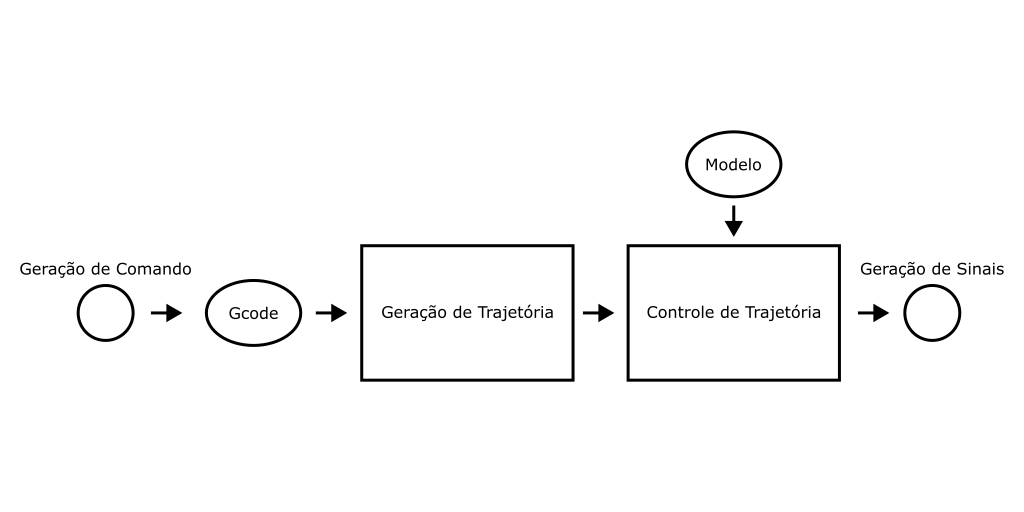
\includegraphics[scale=0.4]{fluxo_geral}

    \label{fig:fluxo_geral}
\end{figure}

\section{Geração de Trajetória}

A fase de geração de trajetória inicia-se com a análise do Gcode, que fornece as coordenadas e velocidades de destino dos movimentos. Neste processo, são considerados exclusivamente os comandos G1, que indicam movimentos lineares, e são extraídas as informações referentes aos eixos X, Y e à taxa de avanço (feedrate - F). É importante notar que a taxa de avanço, usualmente expressa em milímetros por minuto nos arquivos Gcode gerados por fatiadores, é convertida para milímetros por segundo.

\begin{figure}[H]
    \centering
    \caption{Curva de velocidade trapezoidal}
    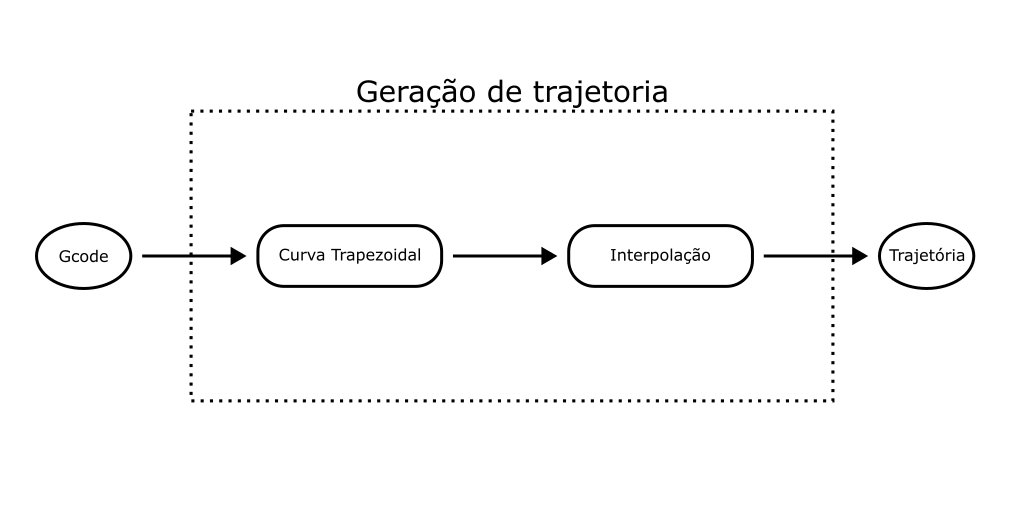
\includegraphics[scale=0.4]{geracao_de_trajetoria}

    \label{fig:geracao_de_trajetoria}
\end{figure}

\subsection{Curva trapezoidal de velocidade}

A próxima etapa  envolve a elaboração da curva trapezoidal de velocidade. Esta etapa se baseia em dados de entrada como deslocamento, velocidades iniciais e finais, e a velocidade almejada. A execução desta velocidade desejada é avaliada através do cálculo da velocidade de pico \(v_p\). Tal velocidade é obtida pela interseção das trajetórias de aceleração e desaceleração, que iniciam nas velocidades iniciais e finais respectivamente, e considerando que a área sob a curva deve ser equivalente ao deslocamento requerido. A fórmula para calcular \(v_p\) é expressa pela Equação \ref{eq:v_p}:

\begin{equation}
    \label{eq:v_p}
    v_p = \sqrt{\frac{(v_1^2+v_2^2)}{2}+a d}
\end{equation}

Nesta equação, \(v_1\) e \(v_2\) representam as velocidades iniciais e finais, \(a\) denota a aceleração definida na impressora, e \(d\) corresponde ao deslocamento.

A comparação entre a velocidade de pico e a velocidade desejada, esta última estabelecida pelo feedrate no Gcode, é crucial para definir se a trajetória do movimento adotará um perfil trapezoidal ou triangular de velocidade. A configuração do perfil depende da relação entre a velocidade de pico e a velocidade desejada: caso a primeira seja superior, o movimento será estruturado em três segmentos distintos, conforme ilustrado na Figura \ref{fig:trap_curv}.

\begin{figure}[H]
    \centering
    \caption{Curva de velocidade trapezoidal}
    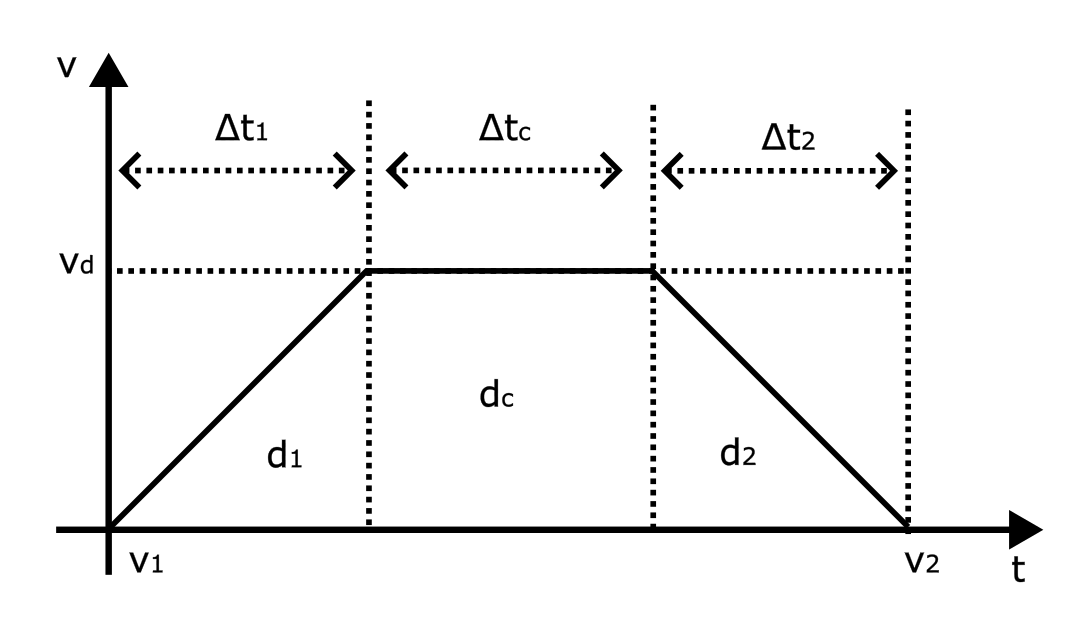
\includegraphics[scale=0.4]{trap_curv}
    \label{fig:trap_curv}
\end{figure}

Os segmentos de deslocamento \(d_1\), \(d_2\), e \(d_c\) correspondem às fases de aceleração, velocidade constante e desaceleração do movimento, respectivamente, e devem totalizar \(d\), o deslocamento total necessário. As variações temporais \(\Delta t_1\), \(\Delta t_2\), e \(\Delta t_c\) representam as durações de cada fase, baseadas nas velocidades inicial (\(v_1\)) e final (\(v_2\)), e na velocidade desejada (\(v_d\)). Os deslocamentos parciais são determinados pelas equações abaixo (Equação \ref{eq:des_seg_1_trap},  \ref{eq:des_seg_2_trap} e  \ref{eq:des_seg_c_trap}), que levam em conta a aceleração \(a\):

\begin{equation}
    \label{eq:des_seg_1_trap}
    d_1 = \frac{(v_d^2-v_1^2)}{(2 a)}
\end{equation}

\begin{equation}
    \label{eq:des_seg_2_trap}
    d_2 = \frac{(v_2^2-v_d^2)}{(2 a)}
\end{equation}

\begin{equation}
    \label{eq:des_seg_c_trap}
    d_c = d-(d_1+d_2)
\end{equation}

Os intervalos de tempo para as fases de aceleração, velocidade constante e desaceleração são calculados conforme (Equação \ref{eq:dt_seg_1_trap},  \ref{eq:dt_seg_2_trap} e  \ref{eq:dt_seg_c_trap}):

\begin{equation}
    \label{eq:dt_seg_1_trap}
    \Delta t_1 = \frac{(v_d-v_1)}{a}
\end{equation}

\begin{equation}
    \label{eq:dt_seg_2_trap}
    \Delta t_2 = \frac{(v_2-v_d)}{a}
\end{equation}

\begin{equation}
    \label{eq:dt_seg_c_trap}
    \Delta t_c = \frac{d_c}{v_d}
\end{equation}

Quando a velocidade de pico (\(v_p\)) é inferior à velocidade desejada (\(v_d\)), o perfil da trajetória de movimento assume uma forma triangular, em vez de trapezoidal. Esta condição implica que a velocidade desejada não é atingida durante o comando e, por conseguinte, o movimento é caracterizado por uma aceleração constante seguida de uma desaceleração constante, sem fase de velocidade constante. A Figura \ref{fig:triang_curv} ilustra este perfil de velocidade triangular.

\begin{figure}[H]
    \centering
    \caption{Curva de velocidade triangular}
    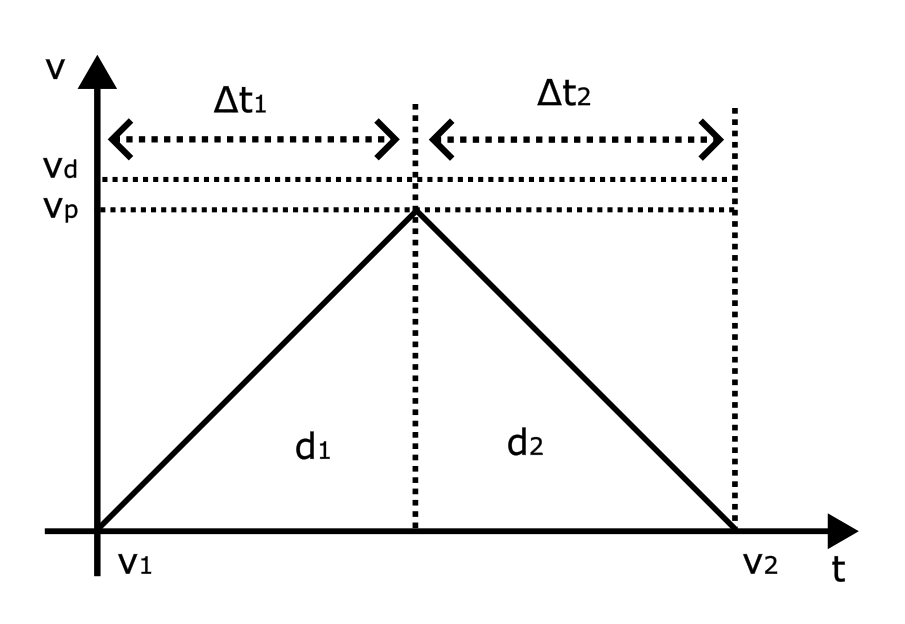
\includegraphics[scale=0.4]{triang_curv}

    \label{fig:triang_curv}
\end{figure}

Neste cenário, os segmentos de deslocamento \(d_1\) e \(d_2\) representam, respectivamente, as etapas de aceleração até a velocidade de pico e a desaceleração de volta à velocidade final. Os valores de \(d_1\) e \(d_2\) são calculados pelas seguintes equações (Equação \ref{eq:des_seg_1_tri}, \ref{eq:des_seg_2_tri}), que incorporam a aceleração (\(a\)) e as velocidades inicial (\(v_1\)) e final (\(v_2\)):

\begin{equation}
    \label{eq:des_seg_1_tri}
    d_1 = \frac{(v_p^2-v_1^2)}{(2 a)}
\end{equation}

\begin{equation}
    \label{eq:des_seg_2_tri}
    d_2 = \frac{(v_2^2-v_p^2)}{(2 a)}
\end{equation}

É possível calcular os intervalos de tempo dessas fases, através das Equações \ref{eq:dt_seg_1_tri} e \ref{eq:dt_seg_2_tri}.

\begin{equation}
    \label{eq:dt_seg_1_tri}
    t_1 = \frac{(v_p-v_1)}{a}
\end{equation}

\begin{equation}
    \label{eq:dt_seg_2_tri}
    t_2 = \frac{(v_2-v_p)}{a}
\end{equation}

Onde os tempos \(t_1\) e \(t_2\) representam, respectivamente, o tempo necessário para acelerar de \(v_1\) a \(v_p\) e para desacelerar de \(v_p\) a \(v_2\). 

Esses passos transformam a sequência de comandos movimentos do Gcode em uma trajetória com pontos com informações do deslocamento, velocidade, tempo, definidos nos nós onde ha alteração na aceleração, estabelecendo o comportamento dos movimentos de x e y no tempo.

\subsection{Interpolação}
A interpolação é um passo crucial para refinar a trajetória de movimento na impressão 3D. Esta fase trabalha sobre a trajetória definida para cada eixo na etapa anterior, empregando uma função de interpolação que gera pontos intermediários. Esses pontos são criados com base em um intervalo de tempo previamente definido, melhorando significativamente a resolução da trajetória.

Para subdividir esses intervalos de maneira eficaz, a Equação \ref{eq:N_steps} é utilizada para calcular o número de passos de interpolação necessários:

\begin{equation}
    \label{eq:N_steps}
    N = \lceil\frac{\Delta t}{\Delta p}-1\rceil
\end{equation}

Esta fórmula determina o número \( N \) de passos a serem tomados dentro de um dado intervalo de tempo \( \Delta t \), com cada passo tendo um período \( \Delta p \). Após a divisão dos intervalos, a Equação \ref{eq:dt_interpol_last_step} calcula o tempo restante no último passo de interpolação (\(\Delta t_f\)):

\begin{equation}
    \label{eq:dt_interpol_last_step}
    \Delta t_f= \Delta t - \Delta p N 
\end{equation}

Finalmente, com base nesses passos de tempo determinados (\(\Delta t_i\)) anexando \(\Delta t_f\) à lista de passos \(\Delta p\) de tamanho \(N\), a Equação \ref{eq:delta_des_interpol} é empregada para calcular o deslocamento correspondente a cada passo (\(\Delta d_i\)), utilizando a aceleração do segmento a ser interpolado (\(a_s\)) e a velocidade inicial do segmento (\(v_s\)):

\begin{equation}
    \label{eq:delta_des_interpol}
    \Delta d_i = \Delta v_s \Delta t_i+ \frac{a_s \Delta t_i^2}{2} 
\end{equation}

Esses cálculos são fundamentais para garantir que a trajetória seja suficientemente detalhada, permitindo que a fase de controle da trajetória seja executada com sucesso.

\section{Modelagem dinâmica de uma impressora 3D} 
\label{sec:modelagem}

A modelagem do sistema mecânico da impressora 3D é um passo crucial para a implementação eficaz do método proposto. Essa modelagem não só facilita a compreensão do comportamento da impressora mas também é fundamental para definir as restrições necessárias na etapa subsequente de controle de trajetória, restrições essas que aplicam as equações de movimento e condições de contorno definidas no modelo.

É fundamental enfatizar a importância de um modelo representativo. A eficácia do método proposto depende diretamente da acurácia com que o modelo simula o comportamento real da impressora 3D. Neste estudo, consideramos as seguintes características principais do sistema (Figura \ref{fig:simple_model}):

\begin{itemize}
    \item Influência da Correia: A correia é o componente chave responsável por introduzir desvios nas trajetórias de impressão. Ela age como uma combinação de mola e amortecedor, afetando a dinâmica do movimento.
    \item Modelagem do Conjunto Bico Injetor e Extrusora: Este conjunto é tratado como um corpo rígido uniforme, simplificando sua representação geométrica. Sua massa é considerada como 200g, o que influencia a dinâmica do movimento.
    \item Dimensões da Mesa de Impressão: A área útil da mesa de impressão é de 200 mm x 200 mm, definindo o espaço de trabalho disponível.
    \item Configuração Cartesiana: A impressora opera em um sistema cartesiano, com eixos ortogonais, o que simplifica a análise de movimento.
    \item Independência dos Eixos: Cada eixo da impressora opera independentemente dos outros, permitindo uma análise mais simplificada das dinâmicas individuais.
    \item Condições Iniciais de Movimento: Assume-se que todos os movimentos da impressora iniciam a partir do estado de repouso.
\end{itemize}

\begin{figure}[H]
    \centering
    \caption{Modelo simplificado impressora 3D}
    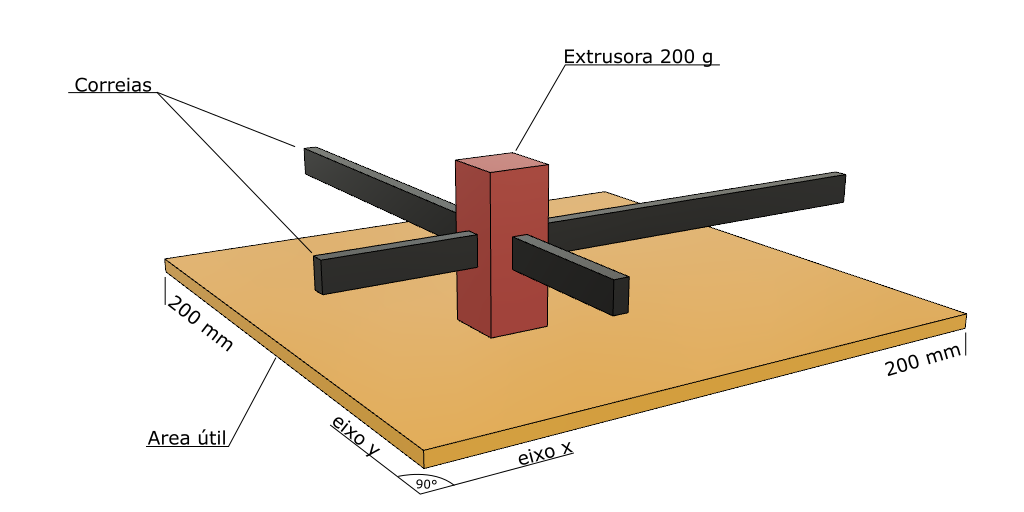
\includegraphics[scale=0.58]{simple_model}
    \label{fig:simple_model}
\end{figure}
Com base nesses parâmetros, definimos duas posições-chave para análise em cada eixo. A primeira é a posição ideal (\(x_b\)) ou posição da base, que representa o ponto desejado pelo usuário, assumindo um sistema sem flexibilidade ou perdas. A segunda é a posição real (\(x_p\)) ou a posição da ponta, que leva em conta as forças inerciais e a flexibilidade introduzida pela correia. Este modelo é ilustrado na figura \ref{fig:model_1_axis}.

\begin{figure}[H]
    \centering
    \caption{Modelagem de 1 eixo}
    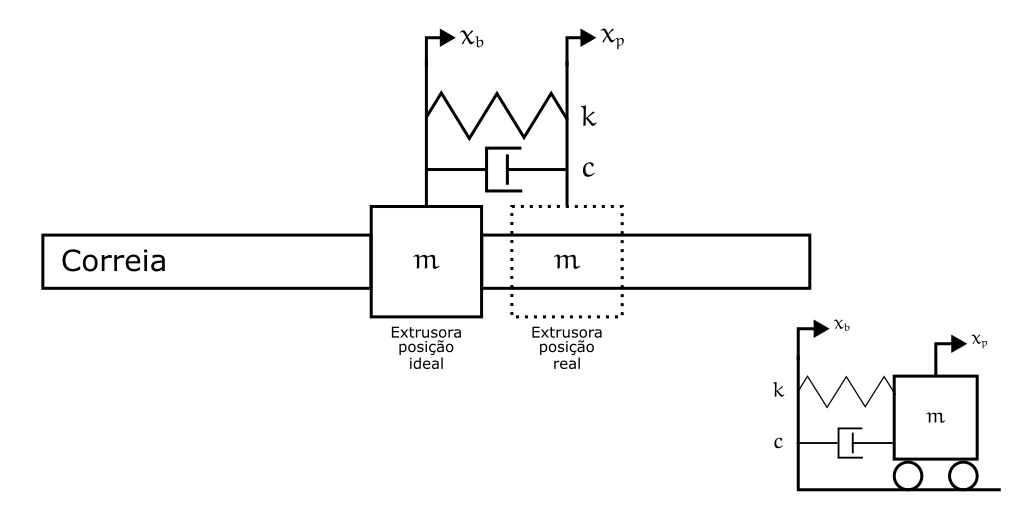
\includegraphics[scale=0.4]{model_1_axis}

    \label{fig:model_1_axis}
\end{figure}

As equações de movimento para a impressora são descritas a seguir:
\begin{multline}
    \label{eq:mov_impressora}
    \\
    m \ddot{x_p} + c(\dot{x_p} - \dot{x_b}) + k(x_p-x_b) = 0 \\
    \ddot{x_p} = - \frac{c}{m} \dot{x_p} - \frac{k}{m} x_p + \frac{c}{m} \dot{x_b} + \frac{k}{m} x_b \\
\end{multline}

Nestas equações, \(m\) representa a massa do conjunto bico injetor e extrusora, \(c\) é a constante de amortecimento da correia, e \(k\) é a constante da mola equivalente da correia. As variáveis \(x_p\) e \(x_b\) correspondem, respectivamente, às posições da ponta e da base do componente em movimento. Essas equações fundamentam o modelo dinâmico que empregamos para simular e otimizar a trajetória de impressão na impressora 3D. Na Figura \ref{fig:model_2_axis} é representada a composição dos eixos x e y utilizado neste estudo, sendo considerada a aplicação das Equação \ref{eq:mov_impressora} para cada um dos eixos de maneira análoga, podendo identificar o eixo através dos subindices \(x\) e \(y\), ou no caso das posições o eixo y é identificado por \(y_p\) e \(y_b\) (posição da ponta do eixo y e posição da base do eixo y respectivamente).

\begin{figure}[H]
    \centering
    \caption{Modelagem dos eixos x e y}
    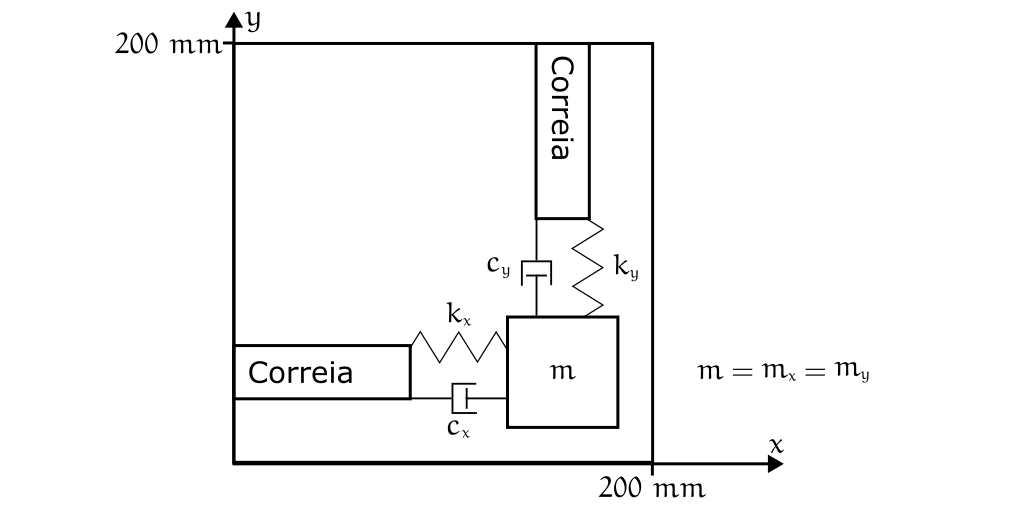
\includegraphics[scale=0.4]{model_2_axis}

    \label{fig:model_2_axis}
\end{figure}

\subsection{Espaço de estados}
A formulação do espaço de estados é adotada neste estudo para simplificar as operações e a solução do sistema dinâmico da impressora 3D. Esta abordagem é eficaz pois transforma uma equação diferencial de ordem superior em um sistema de equações diferenciais de primeira ordem, mas com um número maior de equações. Esta metodologia facilita o entendimento e a manipulação das dinâmicas do sistema.

O modelo dinâmico no espaço de estados é representado na seguinte forma (Equação \ref{eq:simp_state_space_din_model}):

\begin{equation}
    \label{eq:simp_state_space_din_model}
    \dot x = A*x+B*u
\end{equation}

Nesta equação, \(\dot x\) representa o vetor de estados derivados, \(x\) é o vetor de estados, \(A\) é a matriz do sistema que define a relação entre os estados atuais e suas taxas de mudança, \(u\) é o vetor de entradas externas, e \(B\) é a matriz de controle que relaciona as entradas com os estados.

Baseado na equação de movimento \ref{eq:mov_impressora}, análogos ao eixo y, expandimos as matrizes e vetores para representar com precisão a dinâmica do sistema no espaço de estados, conforme apresentado na equação \ref{eq:espaco_de_estados_din_model}:

\begin{equation}
    \label{eq:espaco_de_estados_din_model}
    \begin{bmatrix}
        \dot{x_p} \\
        \ddot{x_p} \\
        \dot{y_p} \\
        \ddot{y_p}
    \end{bmatrix}
    =
    \begin{bmatrix}
        0 & 1 & 0 & 0 \\
        -\frac{k_x}{m_x} & -\frac{c_x}{m_x} & 0 & 0 \\
        0 & 0 & 0 & 1 \\
        0 & 0 & -\frac{k_x}{m_x} & -\frac{c_x}{m_x}
    \end{bmatrix}
    \begin{bmatrix}
        x_p \\
        \dot{x_p} \\        
        y_p \\
        \dot{y_p} \\
    \end{bmatrix}
    +
    \begin{bmatrix}
        0 & 0 & 0 & 0 \\
        \frac{k_x}{m_x} & \frac{c_x}{m_x} & 0 & 0 \\
        0 & 0 & 0 & 0 \\
        0 & 0 & \frac{k_x}{m_x} & \frac{c_x}{m_x}
    \end{bmatrix}
    \begin{bmatrix}
        x_b \\
        \dot{x_b}  \\
        y_b \\
        \dot{y_b} 
    \end{bmatrix}
\end{equation}

Nesta equação, \(x_p\) e \(y_p\) são as posições reais (da ponta) nos eixos X e Y, respectivamente, enquanto \(x_b\) e \(y_b\) são as posições ideais (da base). As variáveis \(\dot{x_p}\) e \(\dot{y_p}\) representam a primeira derivada do tempo das posições nos eixos X e Y, indicando a velocidade e aceleração. \(k_x\) e \(k_y\) denotam as constantes elásticas das correias nos eixos X e Y, enquanto \(c_x\) e \(c_y\) representam as constantes de amortecimento dessas correias. \(m_x\) e \(m_y\) são as massas associadas aos conjuntos de bico injetor e extrusora nos respectivos eixos.

\section{Controle de Trajetória}
O Controle de Trajetória desempenha um papel essencial em aperfeiçoar a precisão dos movimentos na impressora 3D. A escolha das estratégias de controle é crucial para maximizar a eficiência operacional. No escopo deste estudo, a técnica de controle adotada se baseia no modelo estabelecido anteriormente, onde aplicamos uma abordagem feedforward à trajetória gerada na fase de construção da trajetória.

A metodologia de controle em foco procura resolver as equações de movimento e atender às condições de contorno estipuladas pela modelagem da impressora. O ajuste é feito na trajetória da base do sistema, ajustando-a de forma que a saída do vetor de estados corresponda à trajetória da ponta projetada.

Utiliza-se uma função de otimização iterativa para refinar a trajetória da base, que é a principal variável de interesse. Este refinamento é feito minimizando um conjunto de restrições derivadas das equações de movimento e das condições de contorno. A iteração prossegue até que um critério de parada estabelecido seja alcançado, sugerindo que a trajetória base modificada satisfaz a trajetória da ponta almejada.

Este método assegura uma resposta proativa às dinâmicas da impressora, alinhando-se à trajetória planejada e, consequentemente, elevando a acuidade dos movimentos da impressora 3D. A Figura \ref{fig:controle_de_trajetoria} ilustra o esquema do método de controle proposto.

\begin{figure}[H]
    \centering
    \caption{Fluxograma Controle de Trajetória}
    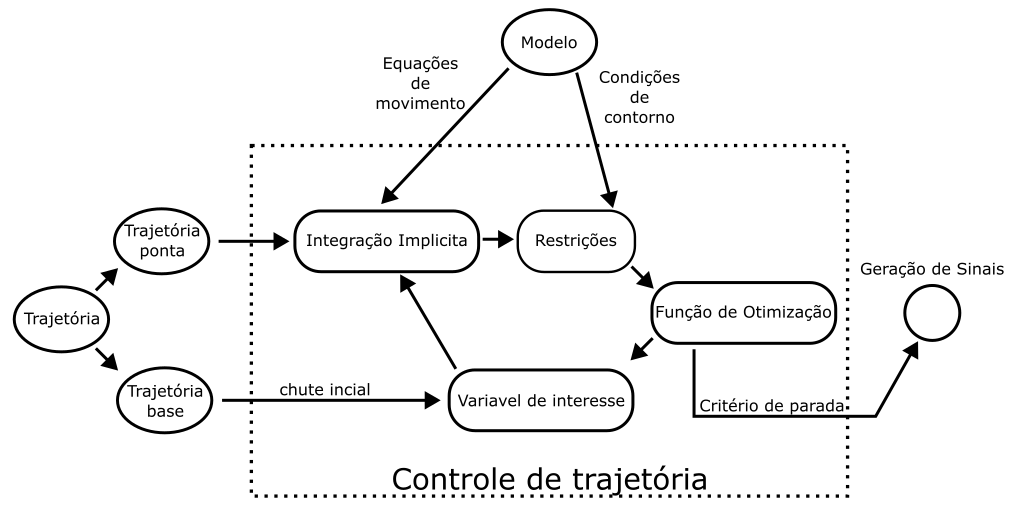
\includegraphics[scale=0.5]{controle_de_trajetoria}

    \label{fig:controle_de_trajetoria}
\end{figure}

\subsection{Restrições}

A formulação do conjunto de restrições é um componente crucial do método, pois é através dele que as equações de movimento são implementadas. A função de otimização adota um algoritmo para minimizar essas restrições, ou seja, para que se aproximem tanto quanto possível de zero.

As condições de contorno são aplicadas estabelecendo que tanto a posição quanto a velocidade sejam zero no instante inicial e que a velocidade também seja zero ao final do percurso. As equações de movimento são incorporadas nas restrições através do método de programação não linear descrito na Seção \ref{sec:hargraves}. Com base no modelo em espaço de estados especificado na Seção \ref{sec:modelagem}. Utilizamos as Equações \ref{eq:state_center_segment}, \ref{eq:state_dot_center_segment}, \ref{eq:input_value_center_segment} e \ref{eq:defect_calc} para criar um vetor de defeitos, como descrito no Capítulo \ref{sec:hargraves}. A minimização destas diferenças faz com que os polinômios cúbicos dos segmentos da curva se aproximem das soluções das equações de movimento, que são então integradas ao vetor de restrições.

\subsection{Função de Otimização}

Os limites da variável de interesse, que neste caso são determinados pela área de trabalho da impressora, também são definidos para que a extrusora não ultrapasse os limites da base de impressão, estabelecendo-se entre o mínimo de 0 e o máximo de 200 mm para os eixos x e y.

A função de otimização adota o algoritmo interior-point, eficaz em resolver problemas de otimização não-linear com restrições. Este método é preferível para grandes conjuntos de dados, por ser mais rápido e numericamente estável do que abordagens tradicionais. Os critérios de parada para o algoritmo são apresentados na Tabela \ref{tab:stop_crit}.

\begin{table}[H]
    \centering
    \caption{Critérios de Parada do Algoritmo de Otimização}
    \label{tab:stop_crit}
    \begin{tabular}{c c}
        Opção & Valor \\ \hline
        Máximo de Iterações & 100000 \\
        Diferença Mínima entre Iterações & 0.0001 \\ \hline
    \end{tabular}
\end{table}

\section{Simulação Computacional e Análise de Dados}

Nesta seção, descrevemos o processo de simulação para testar o método proposto. Iniciamos com a simulação de dois movimentos lineares: um deslocamento de 10 milímetros no eixo x seguido de um movimento similar no eixo y, partindo da posição inicial (0,0) e em estado de repouso. A Figura \ref{fig:base_mov} ilustra estes movimentos.

\begin{figure}[H]
    \centering
    \caption{Movimento base}
    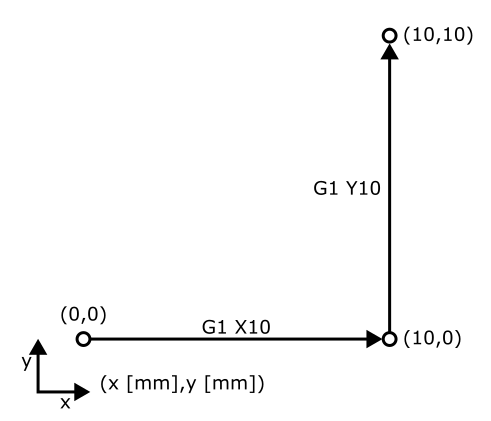
\includegraphics[scale=0.6]{base_mov}

    \label{fig:base_mov}
\end{figure}

Selecionamos parâmetros chave para o controle da simulação, apresentados na Figura \ref{fig:fluxo_geral_var}, e seus respectivos valores são listados na Tabela \ref{tab:base_params}.

\begin{figure}[H]
    \centering
    \caption{Fluxograma geral com os parâmetros.}
    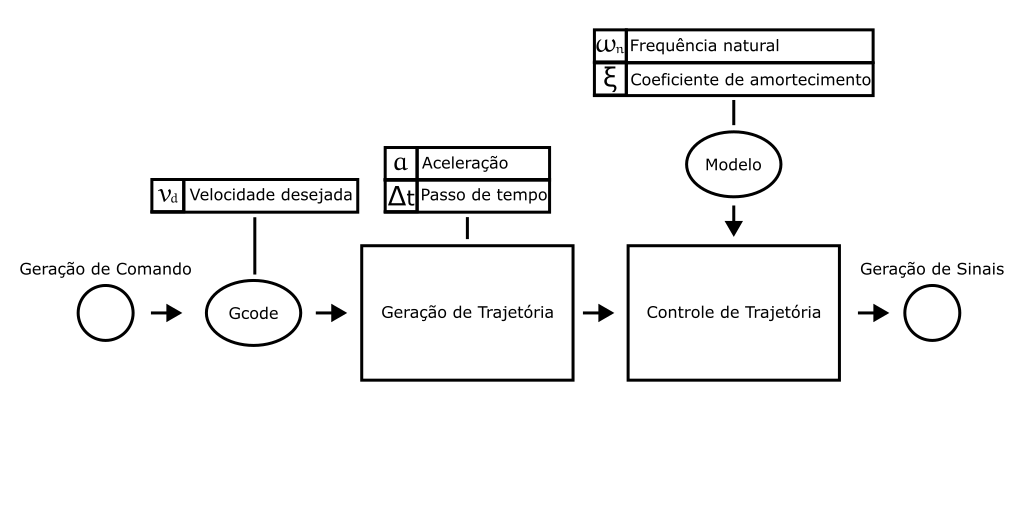
\includegraphics[scale=0.5]{fluxo_geral_var}

    \label{fig:fluxo_geral_var}
\end{figure}

\begin{table}
    \begin{center}
    \caption{Valores dos parâmetros utilizados na simulação.}
    \label{tab:base_params}
    \begin{tabular}{c c c}
        Parâmetro & Valor & Unidade\\ \hline
        Frequência & 100 & $rad/s$\\
        Coeficiente de amortecimento & 0,5 & - \\
        Aceleração base & 5000 & $mm/s^2$ \\
        Passo de tempo & 0,005 & $s$ \\ 
        Velocidade desejada & 100 & $mm/s$ \\ \hline
    \end{tabular}
    \end{center}
\end{table}

Avaliamos a trajetória resultante focando em três aspectos: a viabilidade, o número de iterações e a dimensão do vetor de variáveis de interesse. A viabilidade é medida pelo maior desvio em relação às restrições do modelo, o que nos ajuda a compreender a capacidade da simulação de atingir uma solução que respeite todas as restrições estabelecidas, além de indicar o padrão de convergência ao observar a evolução da viabilidade ao longo das iterações. O tamanho do vetor de variáveis também é considerado, dada a sua relevância para o desempenho computacional da simulação.

\subsection{Análise de Sensibilidade}

Realizamos uma análise de sensibilidade para examinar o comportamento do método frente a variações nos parâmetros listados na Tabela \ref{tab:base_params}. Alteramos cada parâmetro individualmente em 2 ou 3 simulações distintas, conforme detalhado na Tabela \ref{tab:sim_params}. Cada simulação é identificada por um número e uma letra, indicando o parâmetro modificado e o valor aplicado.

\begin{table}
    \begin{center}
    \caption{Parâmetros utilizados na análise de sensibilidade.}
    \label{tab:sim_params}
    \begin{tabular}{c c c c c c}
        Caso & Parâmetro & Valor A & Valor B & Valor C & Unidade\\ \hline
        1 & Frequência & 50 & 200 & 500 & $rad/s$\\
        2 & Coeficiente de amortecimento & 0 & 0,75 & 1 & - \\
        3 & Aceleração base & 1000 & 10000 & - & $mm/s^2$ \\
        4 & Passo de tempo & 0,01 & 0,001 & 0,0002 & $s$ \\
        5 & Velocidade desejada & 50 & 200 & - & $mm/s$ \\ \hline
    \end{tabular}
    \end{center}
\end{table}

As simulações foram executadas em um computador com as especificações listadas na Tabela \ref{tab:note_config}.

\begin{table}
    \begin{center}
    \caption{Especificações do computador}
    \label{tab:note_config}
    \begin{tabular}{c c}
        \hline
        Processador & Intel I7-5500U 2.40GHz \\
        Memoria & 8,00 GB \\
        Placa de vídeo & Nvidia Geforce 920M \\
        Sistema & 64 bits \\ \hline
    \end{tabular}
    \end{center}
\end{table}

\chapter{RESULTADOS E DISCUSSÃO}
Este capítulo detalha os resultados alcançados por meio da análise de sensibilidade aplicada às simulações no estudo do controle de trajetória em impressoras 3D. Essa análise é essencial para avaliar a eficiência do método de controle proposto, considerando sua resposta diante de diferentes condições e parâmetros operacionais. Os resultados destacam a robustez e a viabilidade do método em um contexto real de operação, ao mesmo tempo em que apontam suas possíveis limitações. A apresentação e interpretação dos dados têm como objetivo enfatizar o desempenho do método e oferecer percepções valiosas para futuros avanços e aplicações práticas na área de controle de trajetória para a manufatura aditiva.

Prosseguindo, a análise dos resultados inicia-se com a avaliação da simulação base, estabelecendo um ponto de referência para comparação. Em seguida, detalhamos o impacto e as implicações de cada um dos cinco parâmetros escolhidos na análise de sensibilidade. Estes parâmetros foram criteriosamente selecionados com o objetivo de explorar diferentes aspectos do método de controle e sua resposta em variados cenários operacionais. A investigação destes parâmetros oferece uma visão abrangente sobre como cada elemento influencia o desempenho geral do sistema, permitindo uma compreensão mais profunda e um refinamento do método proposto.

\section{Resultados da Simulação Referência}
Esta seção aborda os resultados obtidos na simulação de referência, com ênfase nas representações gráficas e na metodologia aplicada.

Análise de Velocidades (Figura \ref{fig:t_padr_vels}): Este gráfico exibe as variações das velocidades ao longo do tempo nos eixos X e Y. Ele demonstra a resposta dinâmica tanto da ponta do manipulador quanto da referência estabelecida, conforme a metodologia proposta.

\begin{figure}[H]
    \begin{center}
    \caption{Caso referência - Comportamento no tempo das velocidades em x e y da ponta e da referência}
    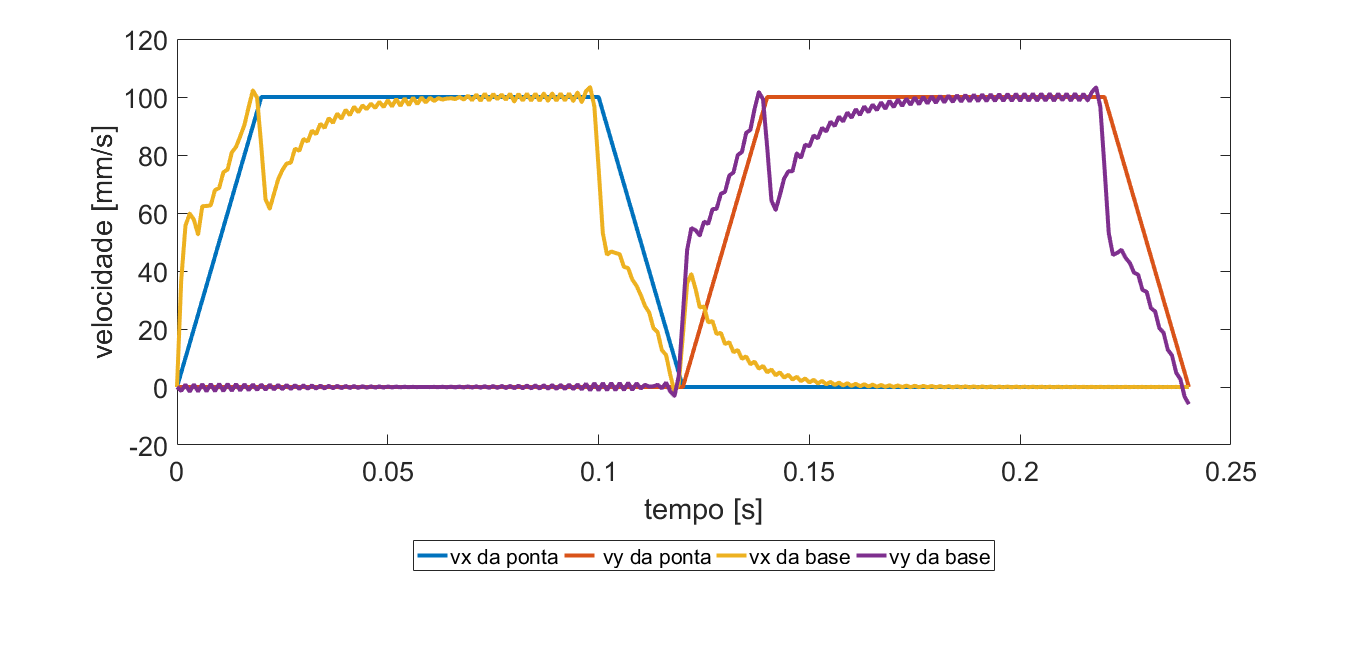
\includegraphics[scale=0.44]{Teste Padrao vels}
    \label{fig:t_padr_vels}
    \end{center}
\end{figure}

Deslocamentos Temporais (Figura \ref{fig:t_padr_des}): Aqui, os deslocamentos nos eixos X e Y são plotados contra o tempo. Esses resultados refletem diretamente a precisão e eficiência do sistema simulado, conforme os critérios estabelecidos na metodologia.

\begin{figure}[H]
    \begin{center}
    \caption{Caso referência - Comportamento no tempo dos deslocamentos em x e y da ponta e da referência}
    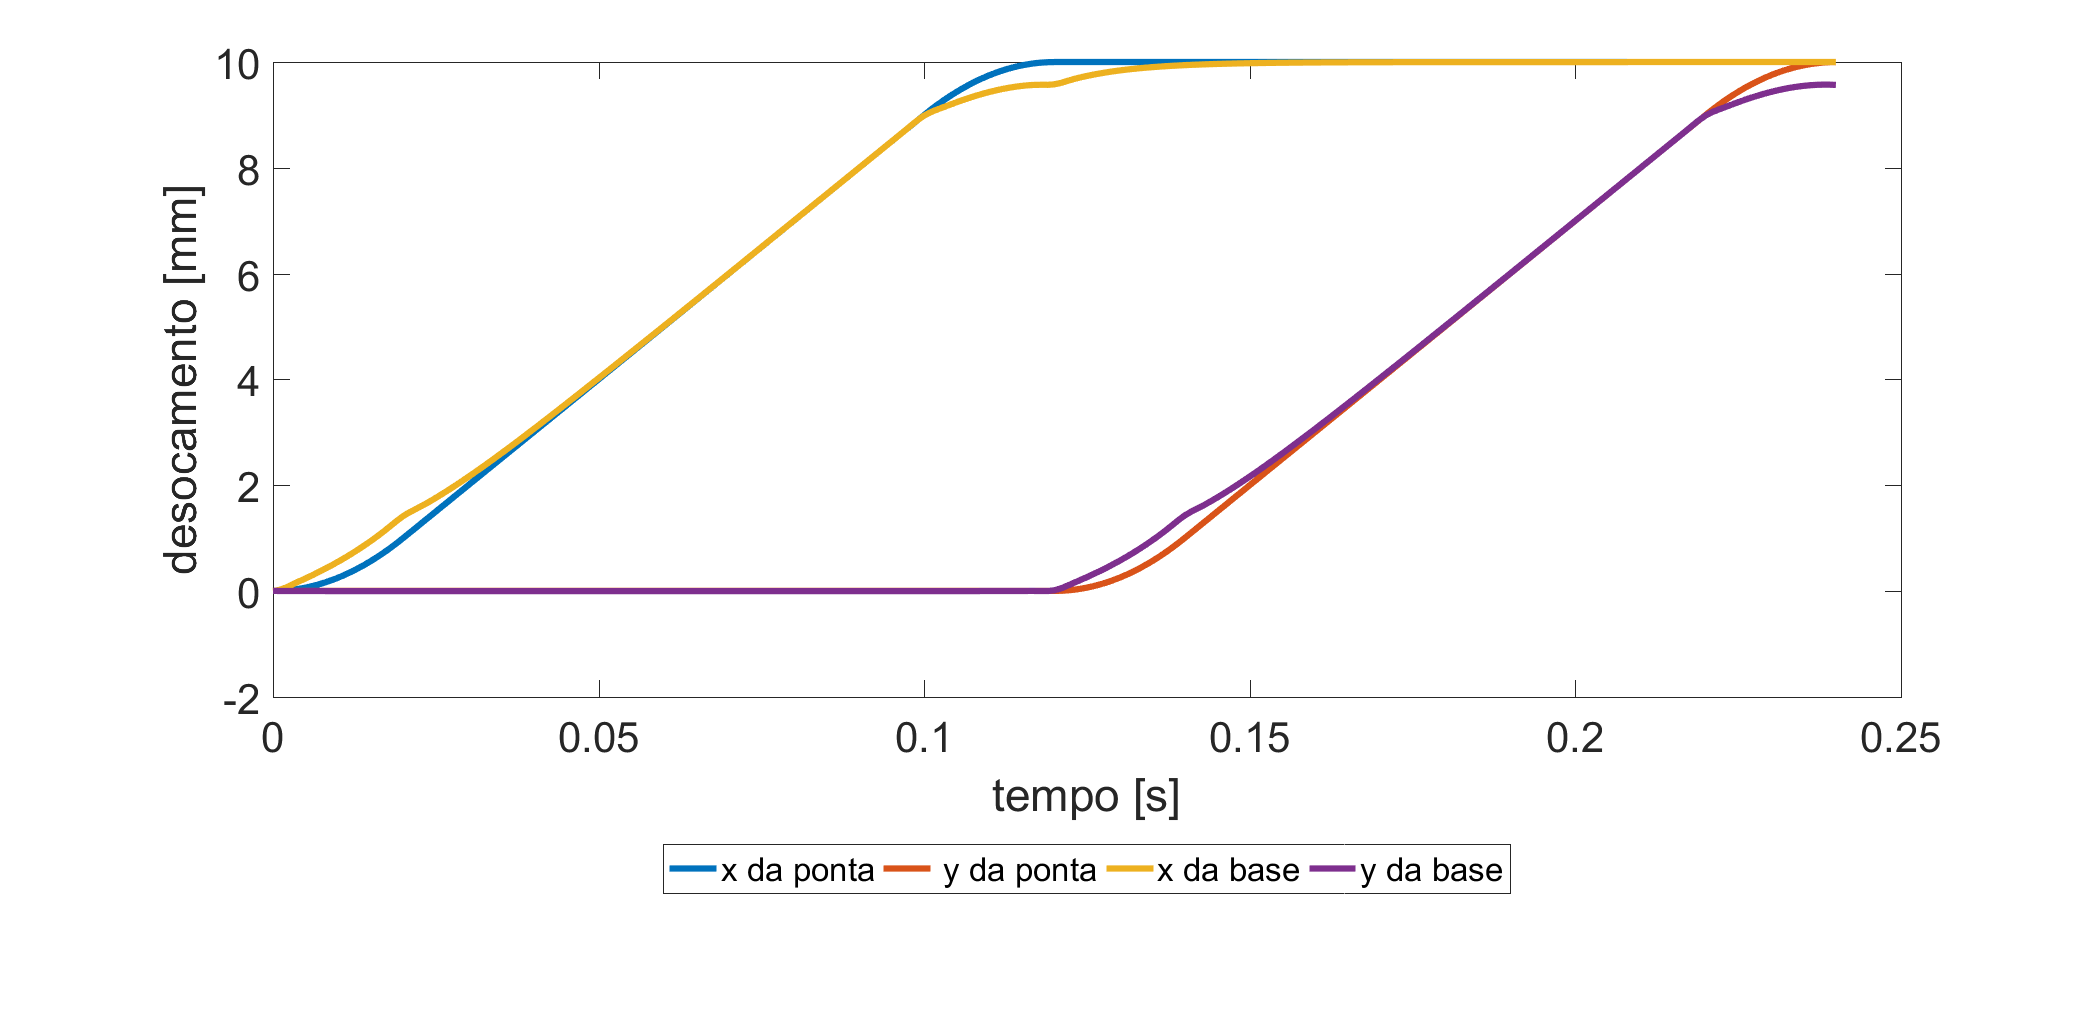
\includegraphics[scale=0.44]{Teste Padrao des}
    \label{fig:t_padr_des}
    \end{center}
\end{figure}    

Trajetória Espacial (Figura \ref{fig:t_padr_pos}): Este gráfico ilustra o caminho percorrido nos planos X e Y, comparando a trajetória da ponta com a trajetória de referência. A aderência ao caminho planejado, conforme descrito na metodologia, é fundamental para avaliar a acurácia do sistema.

\begin{figure}[H]
    \begin{center}
    \caption{Caso referência - Caminho percorrido x vs y da ponta e da referência}
    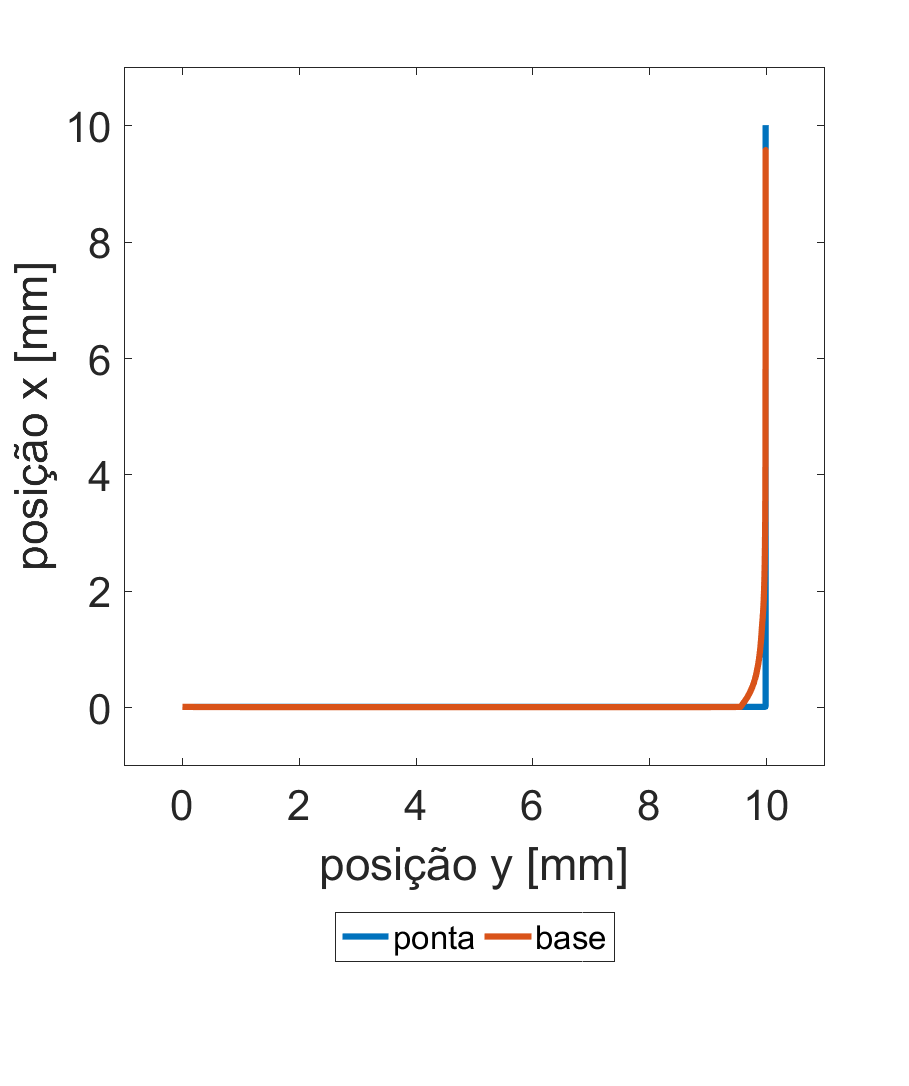
\includegraphics[scale=0.44]{Teste Padrao pos}
    \label{fig:t_padr_pos}
    \end{center}
\end{figure}

O gráfico apresentado na Figura \ref{fig:t_padr_viab} exibe a evolução das iterações durante a simulação. Cada ponto no gráfico representa uma iteração distinta. O eixo X mostra o número de avaliações da função objetivo e das restrições, enquanto o eixo Y reflete o valor de viabilidade, que indica o grau de cumprimento das restrições mais desafiadoras, conforme discutido na metodologia.

Observa-se uma tendência clara de convergência ao longo das iterações, um indicativo de que a simulação está alcançando resultados bem-sucedidos. Notavelmente, os valores iniciais de viabilidade se aproximam de $7,5x10^{-3}$, um padrão consistente observado em vários casos.

Além disso, o tempo total de simulação para esta análise foi de aproximadamente 89,8 segundos. Os vetores de posição empregados na simulação contavam com 241 elementos, refletindo a complexidade e a precisão dos cálculos realizados.

Este gráfico é fundamental para entender a eficácia da simulação em atender às restrições estabelecidas e a capacidade do sistema de convergir para uma solução viável em um tempo eficiente.

\begin{figure}[H]
    \begin{center}
    \caption{Caso referência - Num de fun x Viabilidade}
    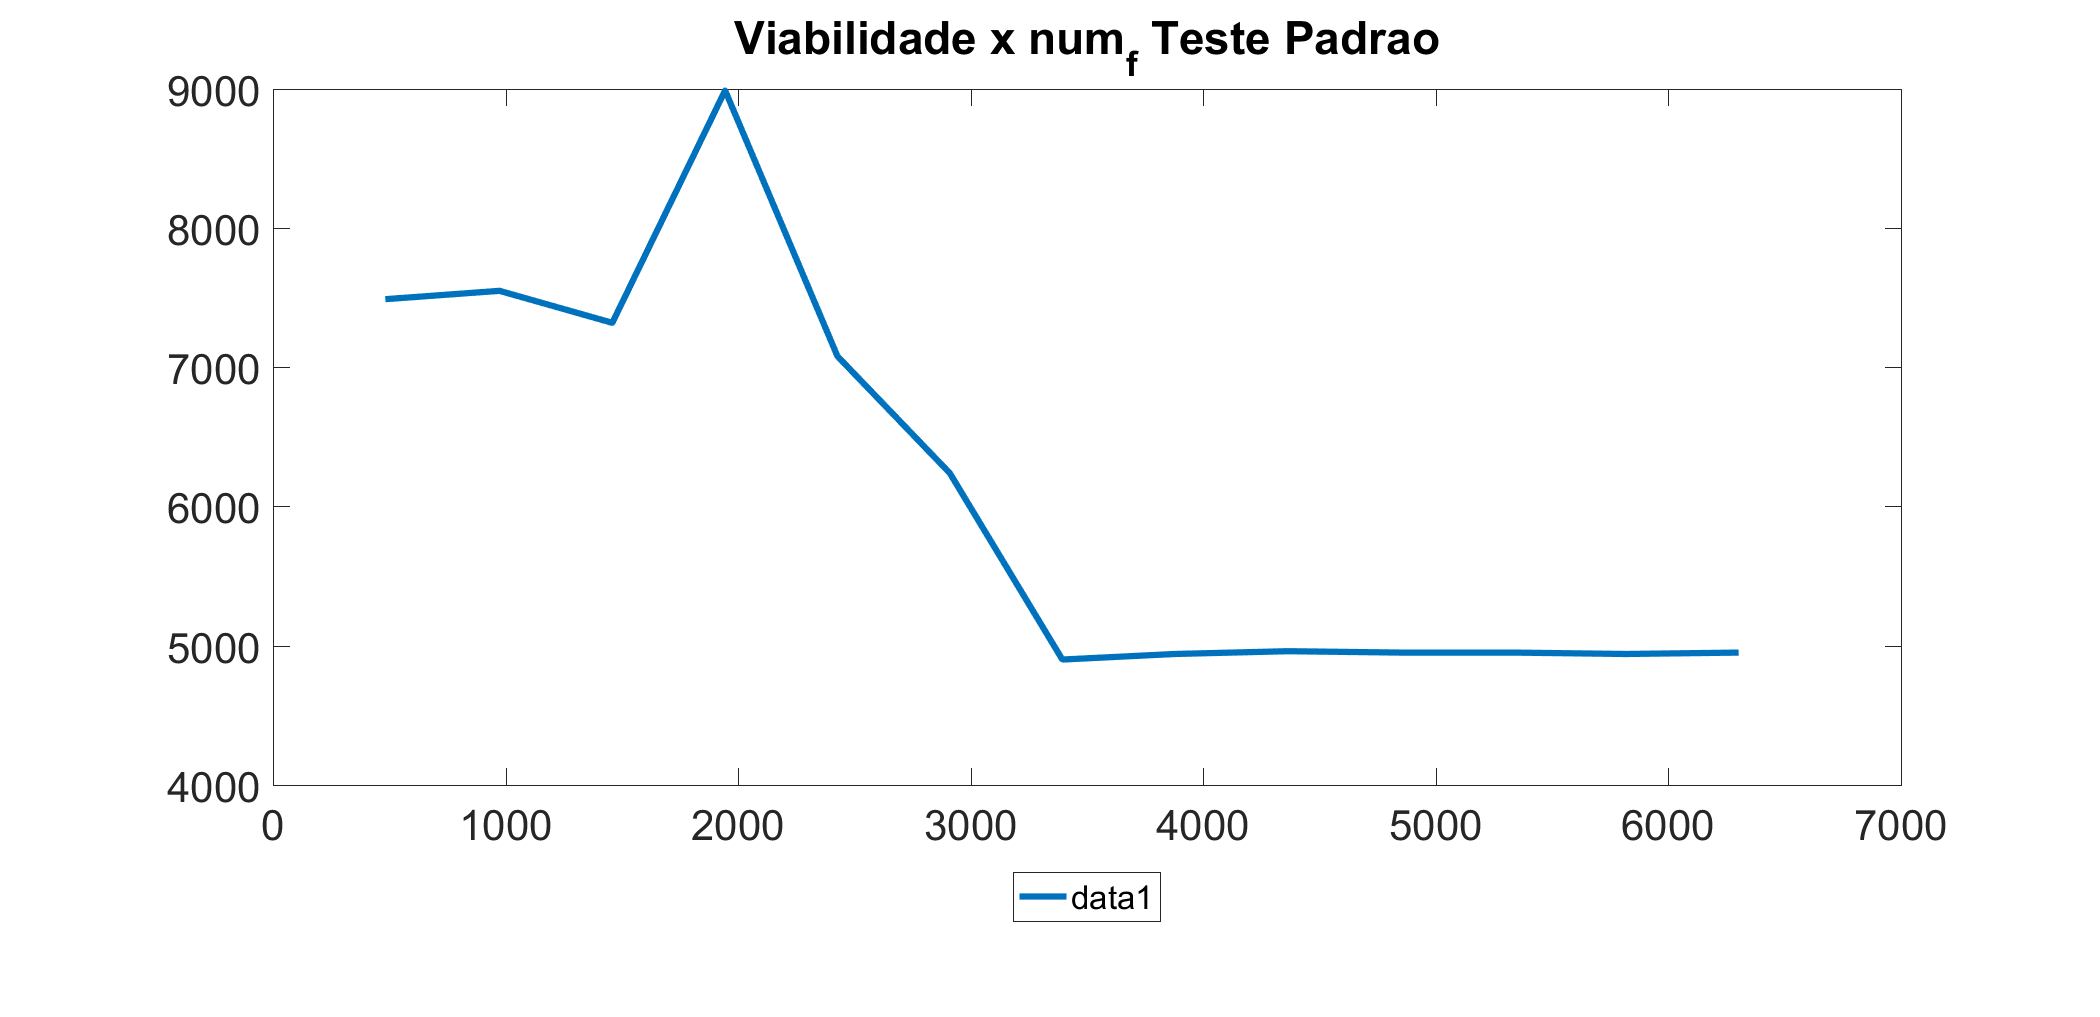
\includegraphics[scale=0.44]{Teste Padrao Viabilidade}
    \label{fig:t_padr_viab}
    \end{center}
\end{figure}

\section{Análise de Sensibilidade dos Resultados}
\subsection{Caso 1 - Variação da frequência}
Este caso investiga como a variação da frequência natural afeta o modelo dinâmico do sistema. A frequência natural, sendo um parâmetro crítico, influencia diretamente o comportamento da planta do modelo, com implicações notáveis nas amplitudes dos desvios e na necessidade de compensação.

Observamos que sistemas com maior rigidez, caracterizados por frequências naturais mais altas, exibem menores amplitudes de desvio e uma reduzida necessidade de compensação. Esta tendência é claramente ilustrada ao comparar as figuras \ref{fig:t_1a_vels}, \ref{fig:t_1b_vels} e \ref{fig:t_1c_vels}, que mostram o comportamento das velocidades em x e y para diferentes configurações de frequência.

\begin{figure}[H]
    \begin{center}
    \caption{Caso 1A - Comportamento no tempo das velocidades em x e y da ponta e da referência}
    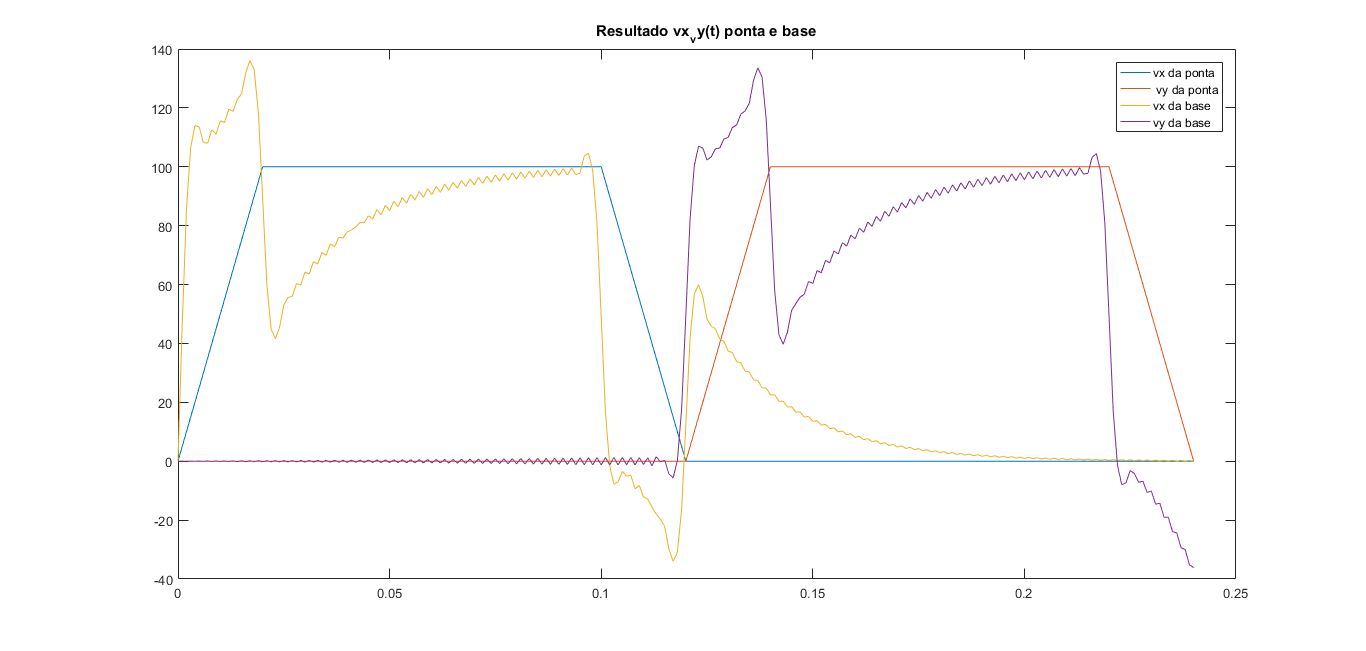
\includegraphics[scale=0.44]{Teste 1 A vels}
    \label{fig:t_1a_vels}
    \end{center}
\end{figure}

\begin{figure}[H]
    \begin{center}
    \caption{Caso 1B - Comportamento no tempo das velocidades em x e y da ponta e da referência}
    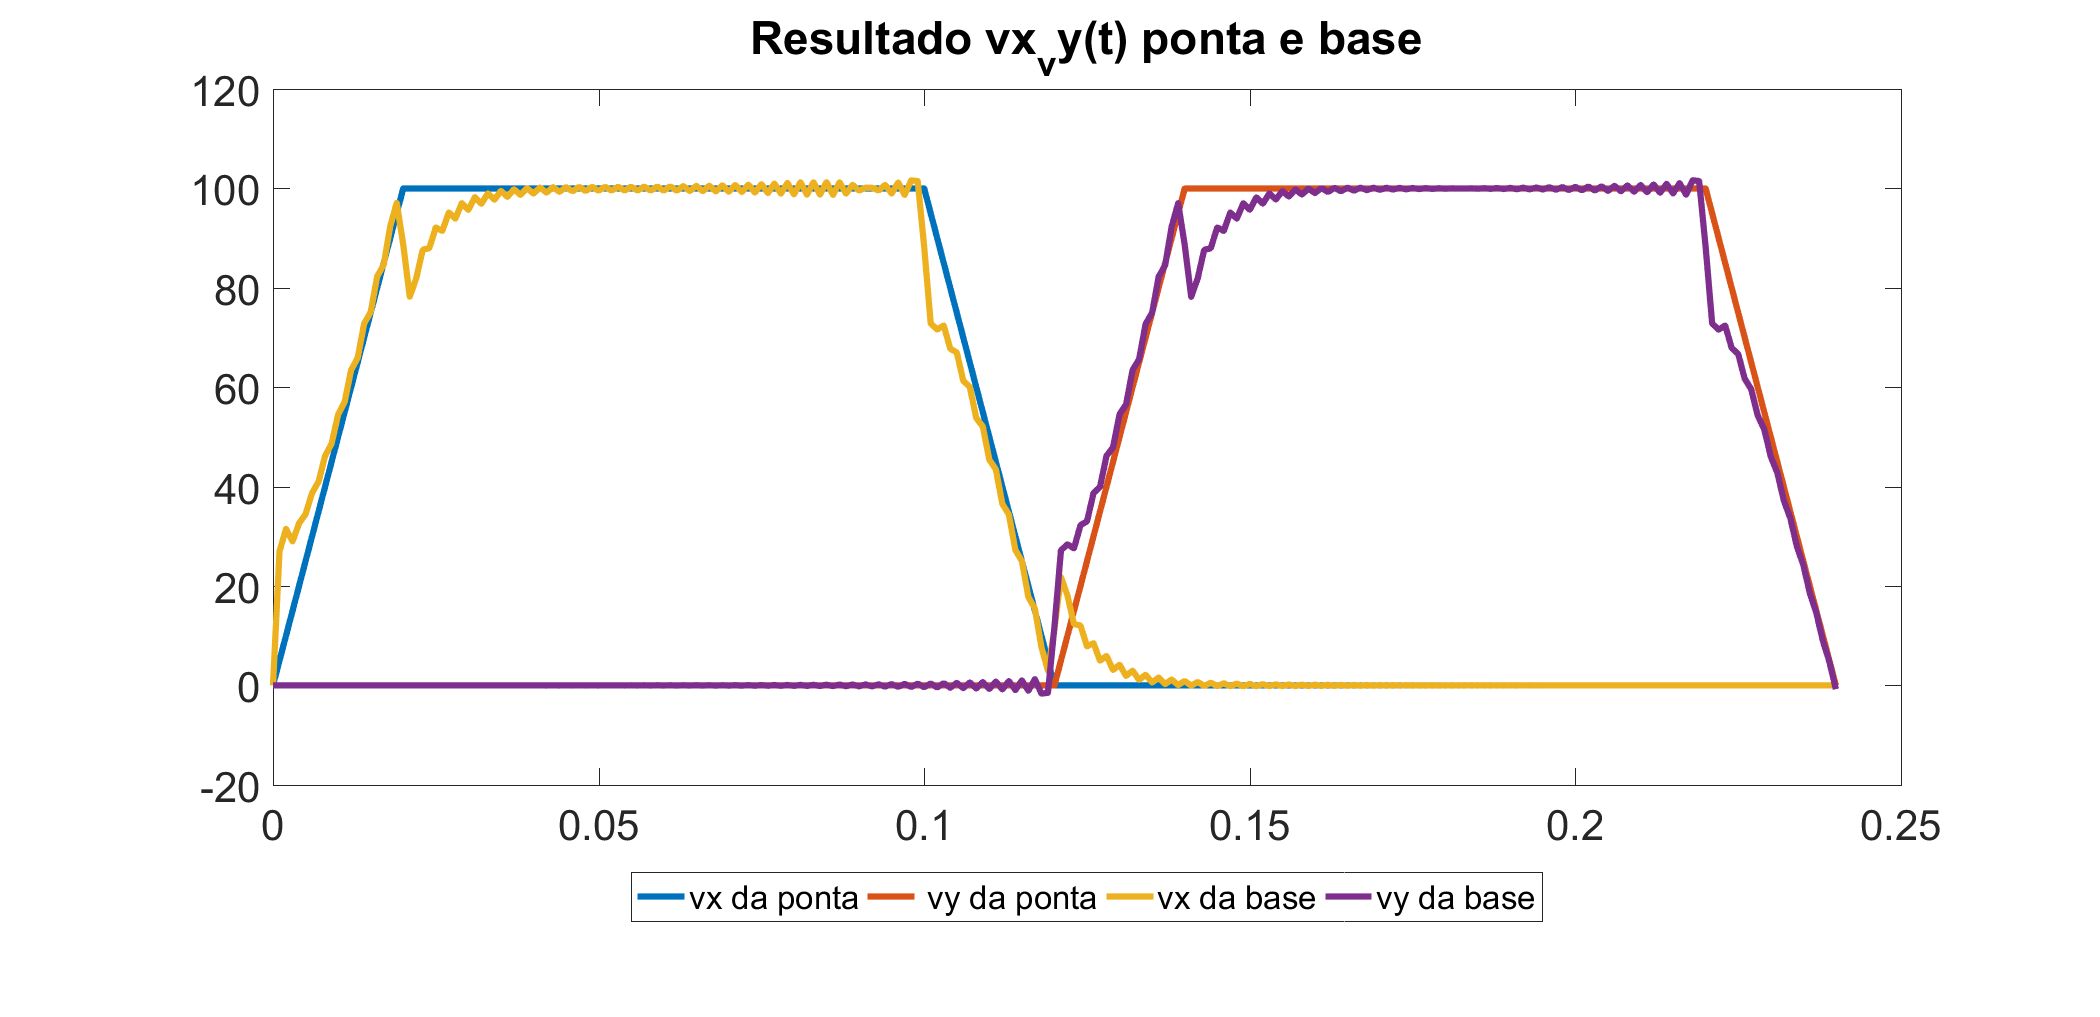
\includegraphics[scale=0.44]{Teste 1 B vels}
    \label{fig:t_1b_vels}
    \end{center}
\end{figure}

\begin{figure}[H]
    \begin{center}
    \caption{Caso 1C - Comportamento no tempo das velocidades em x e y da ponta e da referência}
    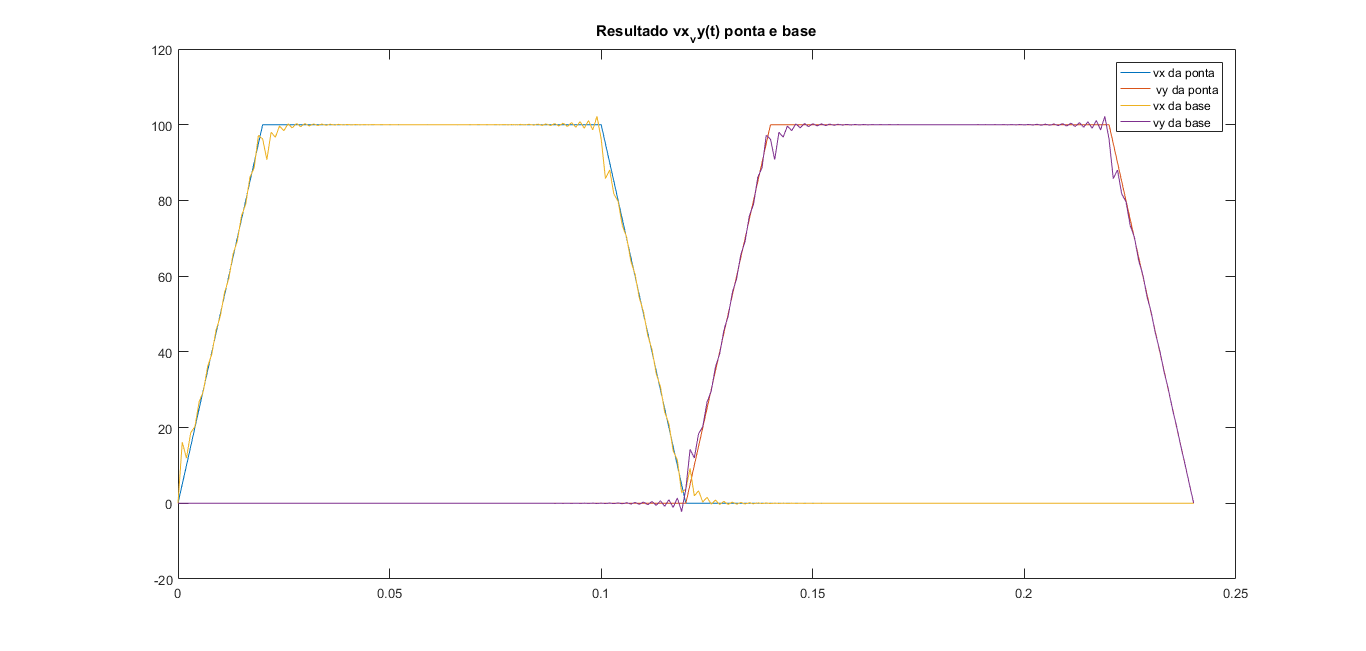
\includegraphics[scale=0.44]{Teste 1 C vels}
    \label{fig:t_1c_vels}
    \end{center}
\end{figure}

A análise é aprofundada ao examinar as figuras \ref{fig:t_1a_des}, \ref{fig:t_1c_des}, \ref{fig:t_1a_pos} e \ref{fig:t_1c_pos}, que revelam as diferenças no comportamento do deslocamento e no caminho percorrido pela ponta do sistema nos extremos do caso (A e C). Estes resultados indicam que variações na frequência natural não apenas afetam as propriedades dinâmicas, mas também têm implicações diretas no controle e precisão do sistema.

\begin{figure}[H]
    \begin{center}
    \caption{Caso 1A - Comportamento no tempo dos deslocamentos em x e y da ponta e da referência}
    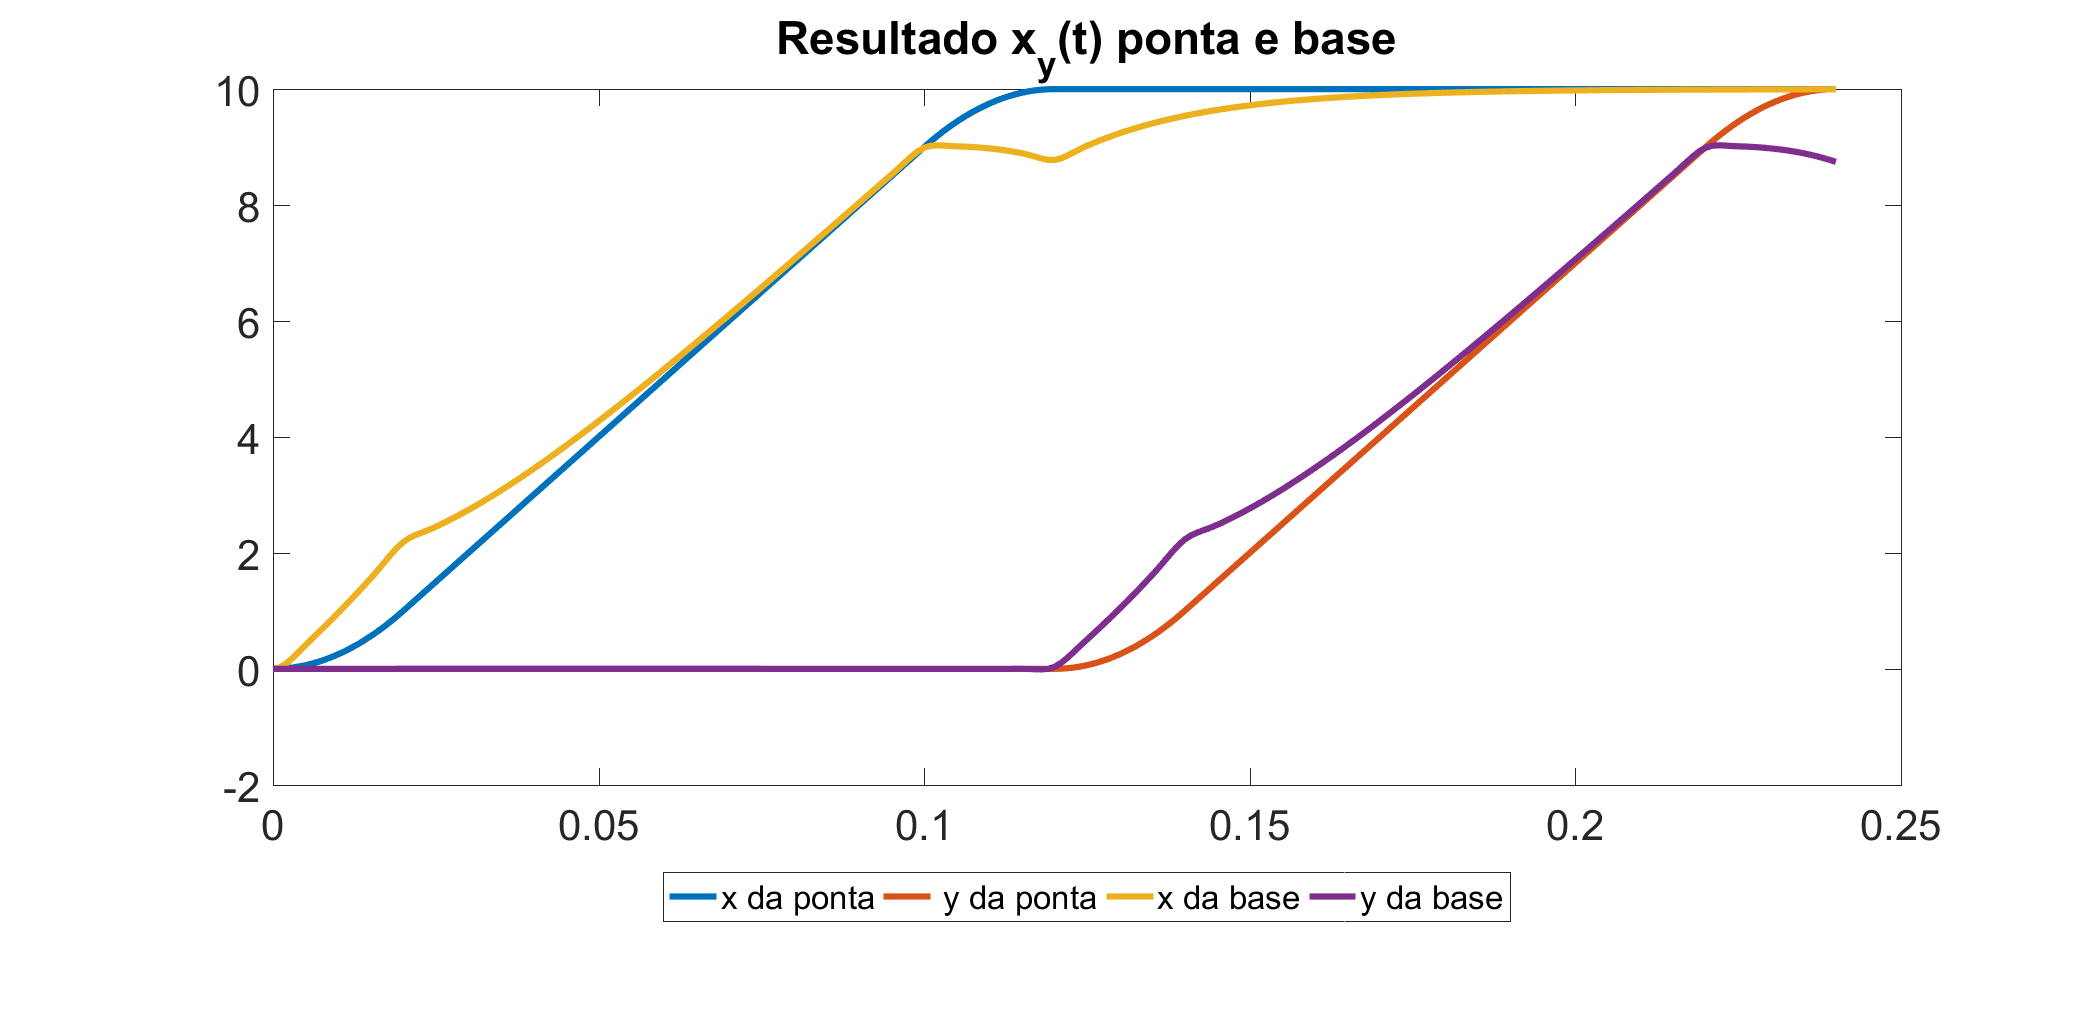
\includegraphics[scale=0.44]{Teste 1 A des}
    \label{fig:t_1a_des}
    \end{center}
\end{figure}

\begin{figure}[H]
    \begin{center}
    \caption{Caso 1C - Comportamento no tempo dos deslocamentos em x e y da ponta e da referência}
    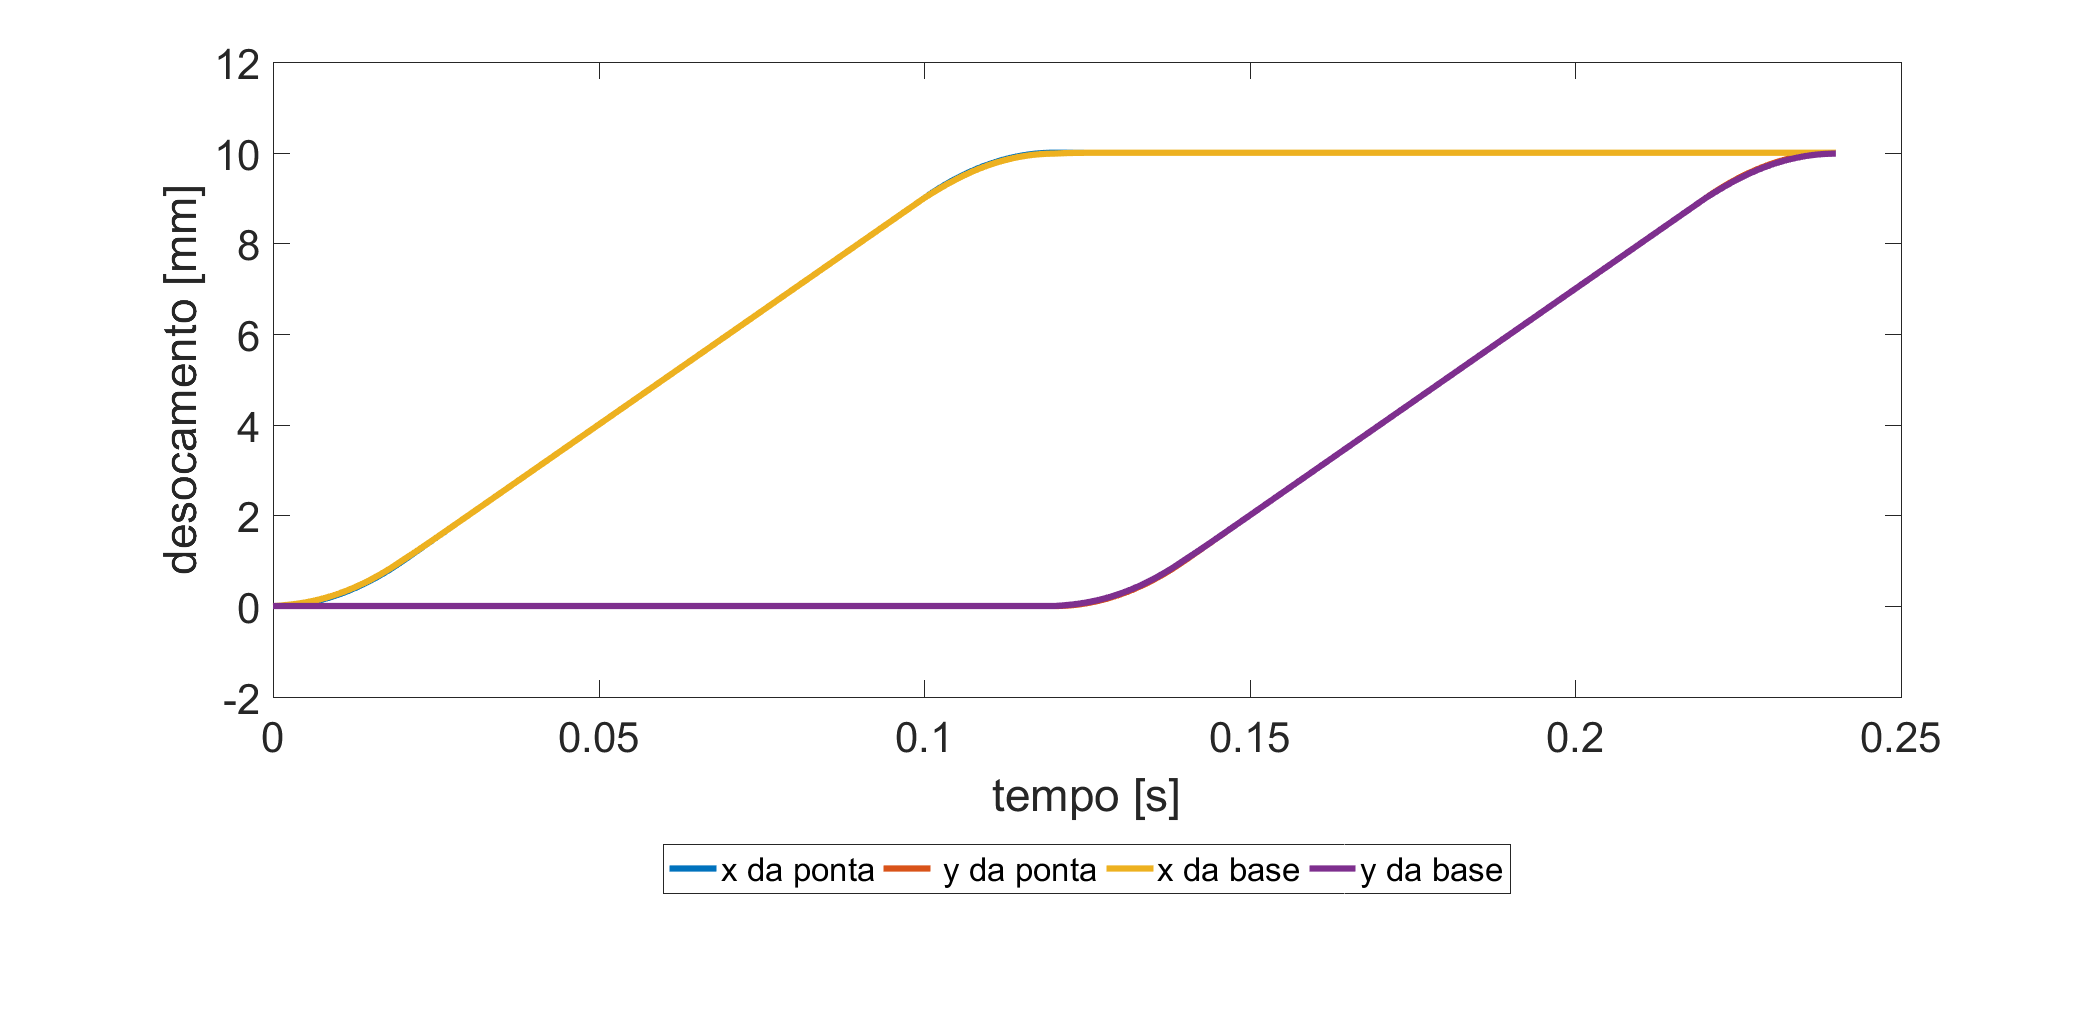
\includegraphics[scale=0.44]{Teste 1 C des}
    \label{fig:t_1c_des}
    \end{center}
\end{figure}

\begin{figure}[H]
    \begin{center}
    \caption{Caso 1A - Caminho percorrido x vs y da ponta e da referência}
    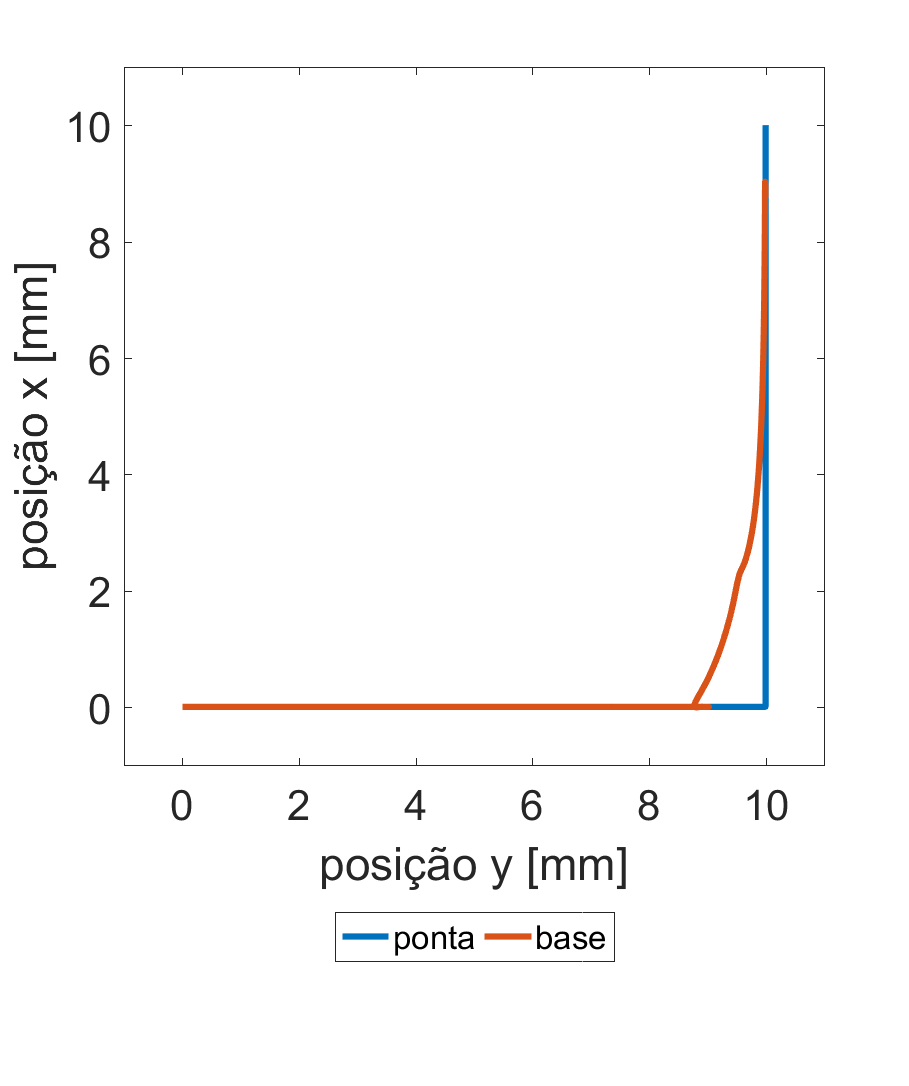
\includegraphics[scale=0.44]{Teste 1 A pos}
    \label{fig:t_1a_pos}
    \end{center}
\end{figure}

\begin{figure}[H]
    \begin{center}
    \caption{Caso 1C - Caminho percorrido x vs y da ponta e da referência}
    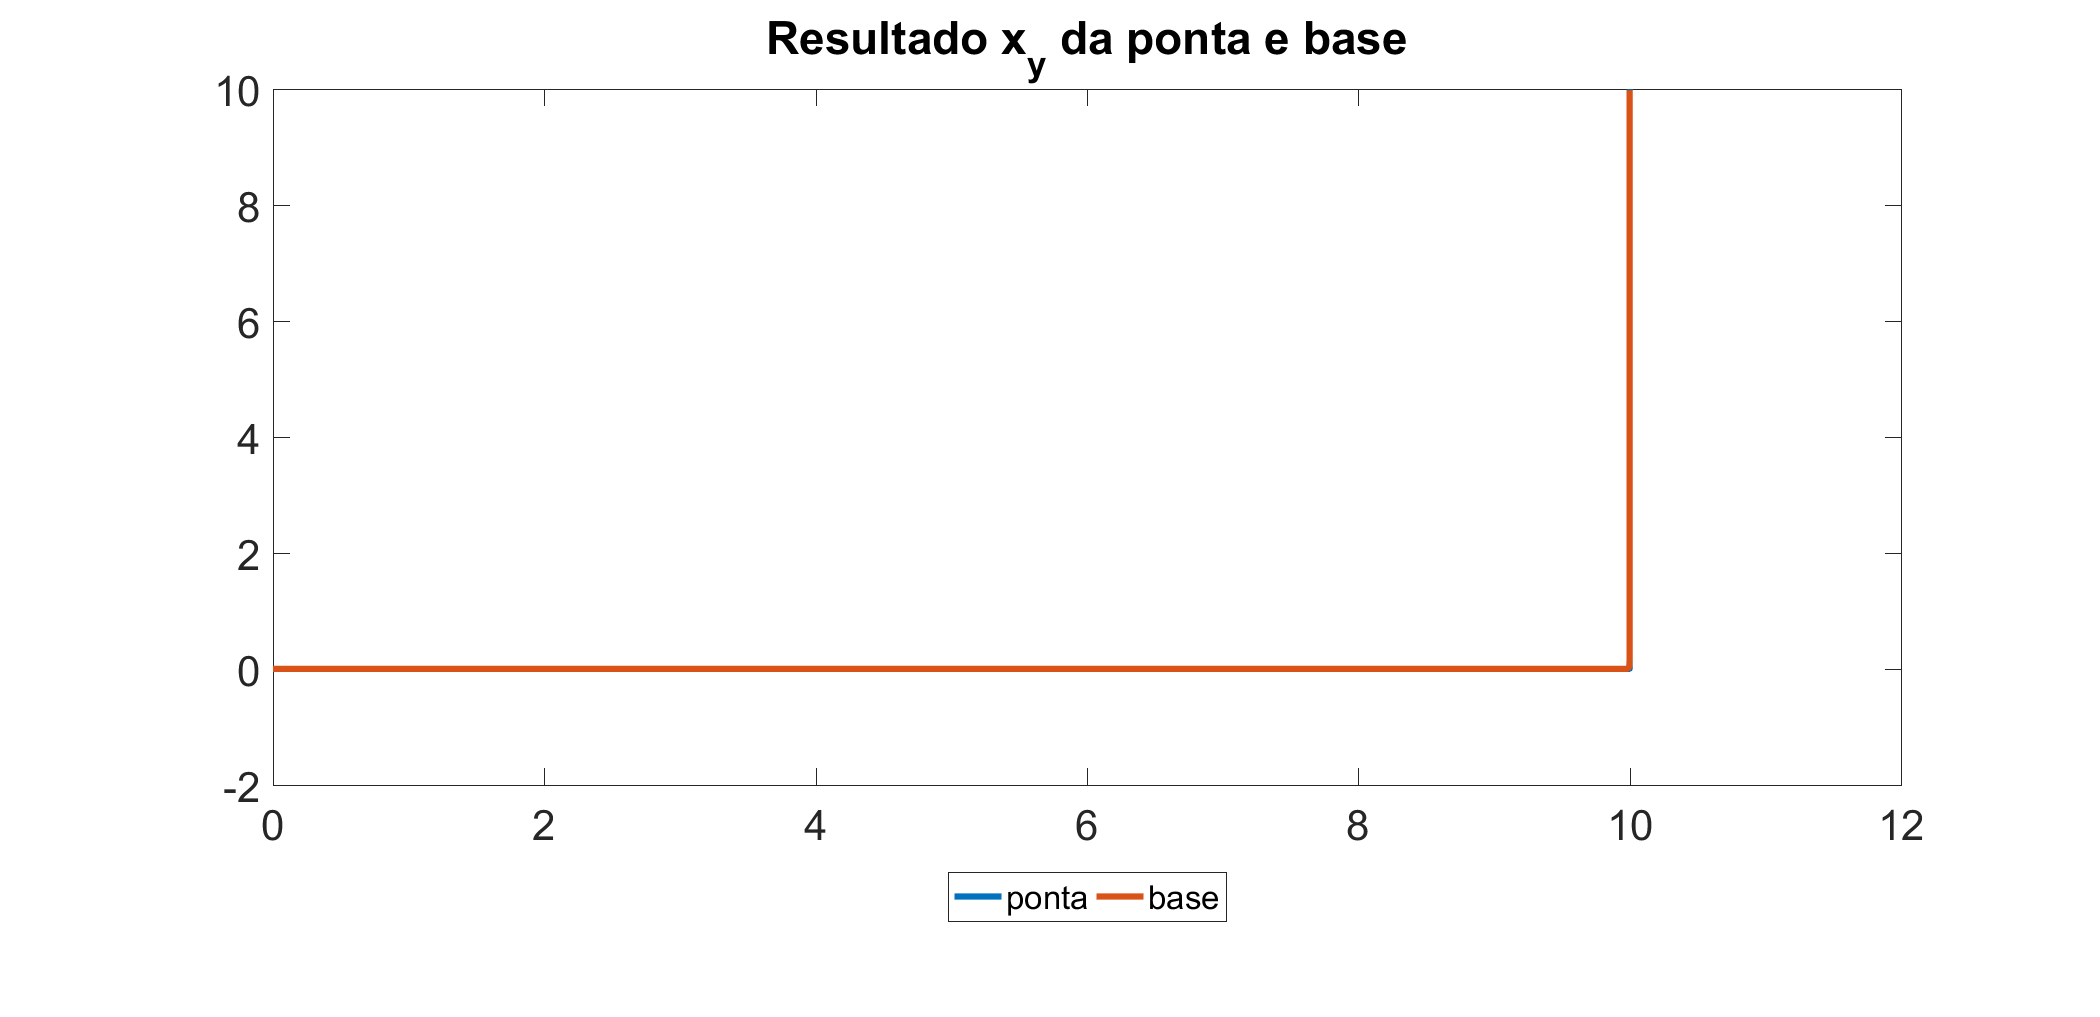
\includegraphics[scale=0.44]{Teste 1 C pos}
    \label{fig:t_1c_pos}
    \end{center}
\end{figure}

Além disso, a figura \ref{fig:t_1_viab} fornece uma visão geral da viabilidade do sistema sob diferentes configurações de frequência natural. Observamos um padrão de convergência similar em todos os casos, mas com uma viabilidade menor e, consequentemente, menores violações das restrições impostas nos casos de maior rigidez. Isso reflete um equilíbrio mais eficiente entre precisão e esforço computacional.

\begin{figure}[H]
    \begin{center}
    \caption{Caso 1 - Num de fun x Viabilidade}
    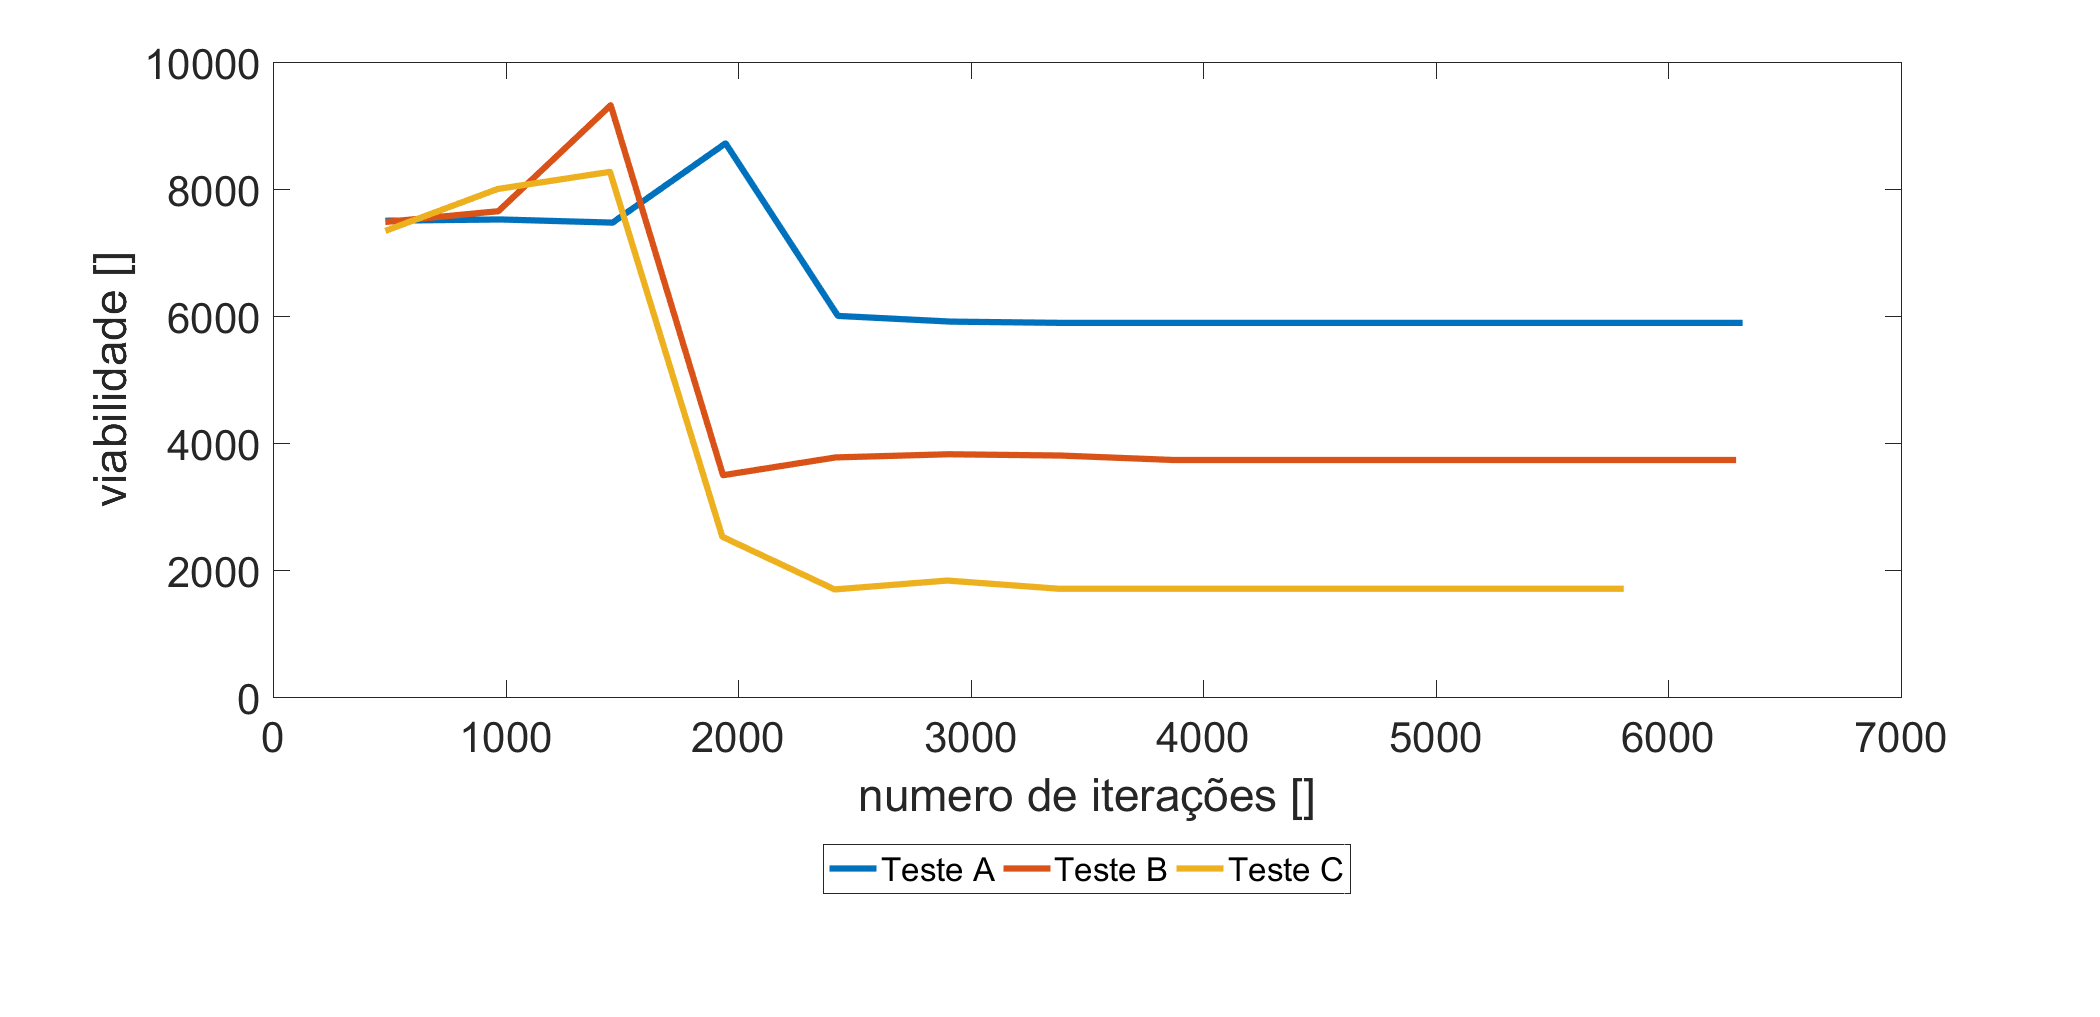
\includegraphics[scale=0.44]{Teste 1 Viabilidade}
    \label{fig:t_1_viab}
    \end{center}
\end{figure}

Importante também é o impacto dessas variações na frequência natural no tempo de simulação. Observamos que os tempos de simulação variaram de 96,76 segundos no Caso A até 80,77 segundos no Caso C, com o Caso B intermediário, em 89,04 segundos. Esta tendência sugere que sistemas com maior rigidez (frequências naturais mais altas) não apenas melhoram a eficácia em termos de cumprimento das restrições, mas também podem levar a uma simulação mais rápida, apesar de todos os casos utilizarem vetores de posição com 241 elementos. Esta observação é crítica para aplicações práticas, onde a eficiência computacional e a rapidez na resposta são essenciais.

\subsection{Caso 2 - Variação do coeficiente de amortecimento}
Neste caso, investigamos o impacto de diferentes coeficientes de amortecimento no comportamento do sistema. As Figuras \ref{fig:t_2b_pos} e \ref{fig:t_2c_pos} são cruciais para esta análise, pois ilustram as trajetórias espaciais para as variações B e C do coeficiente de amortecimento. Estes resultados são contrastados com a Figura \ref{fig:t_padr_pos}, que representa um coeficiente intermediário, oferecendo uma comparação direta entre os extremos e o caso base.

\begin{figure}[H]
    \begin{center}
    \caption{Caso 2B - Caminho percorrido x vs y da ponta e da referência}
    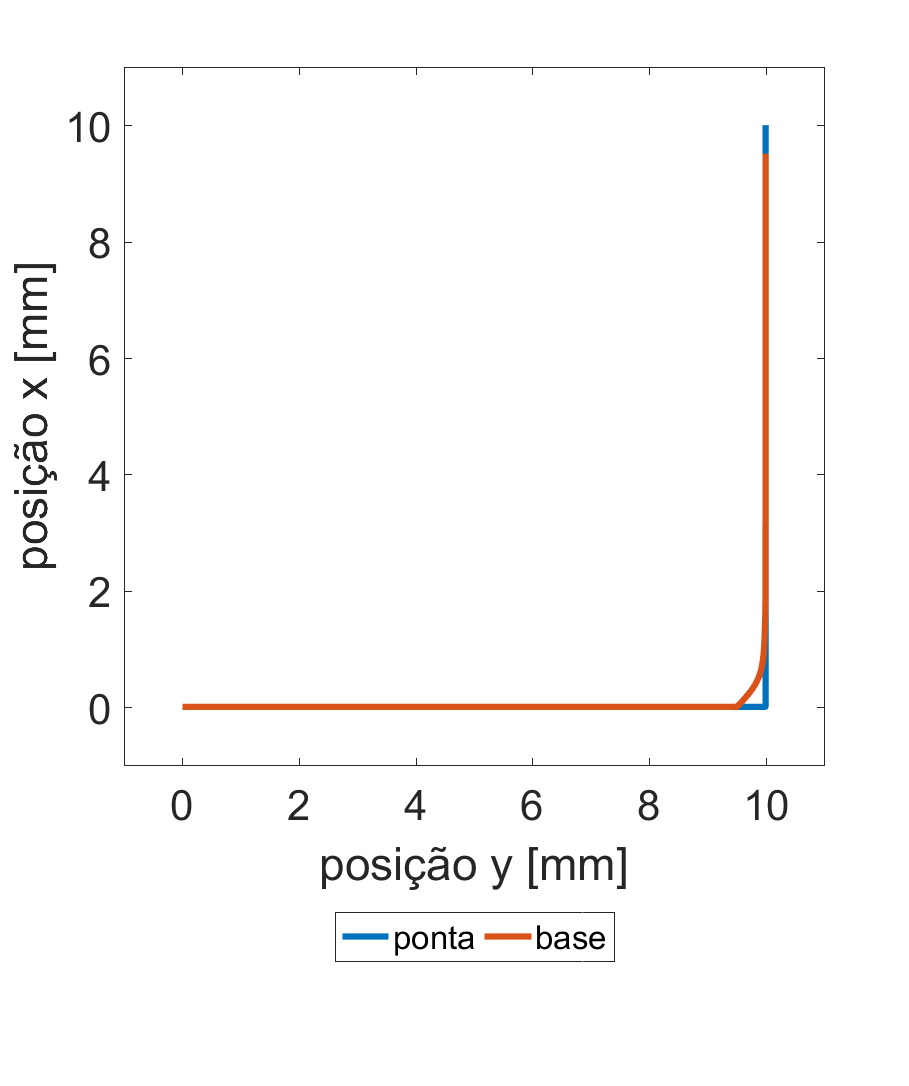
\includegraphics[scale=0.44]{Teste 2 B pos}
    \label{fig:t_2b_pos}
    \end{center}
\end{figure}

\begin{figure}[H]
    \begin{center}
    \caption{Caso 2C - Caminho percorrido x vs y da ponta e da referência}
    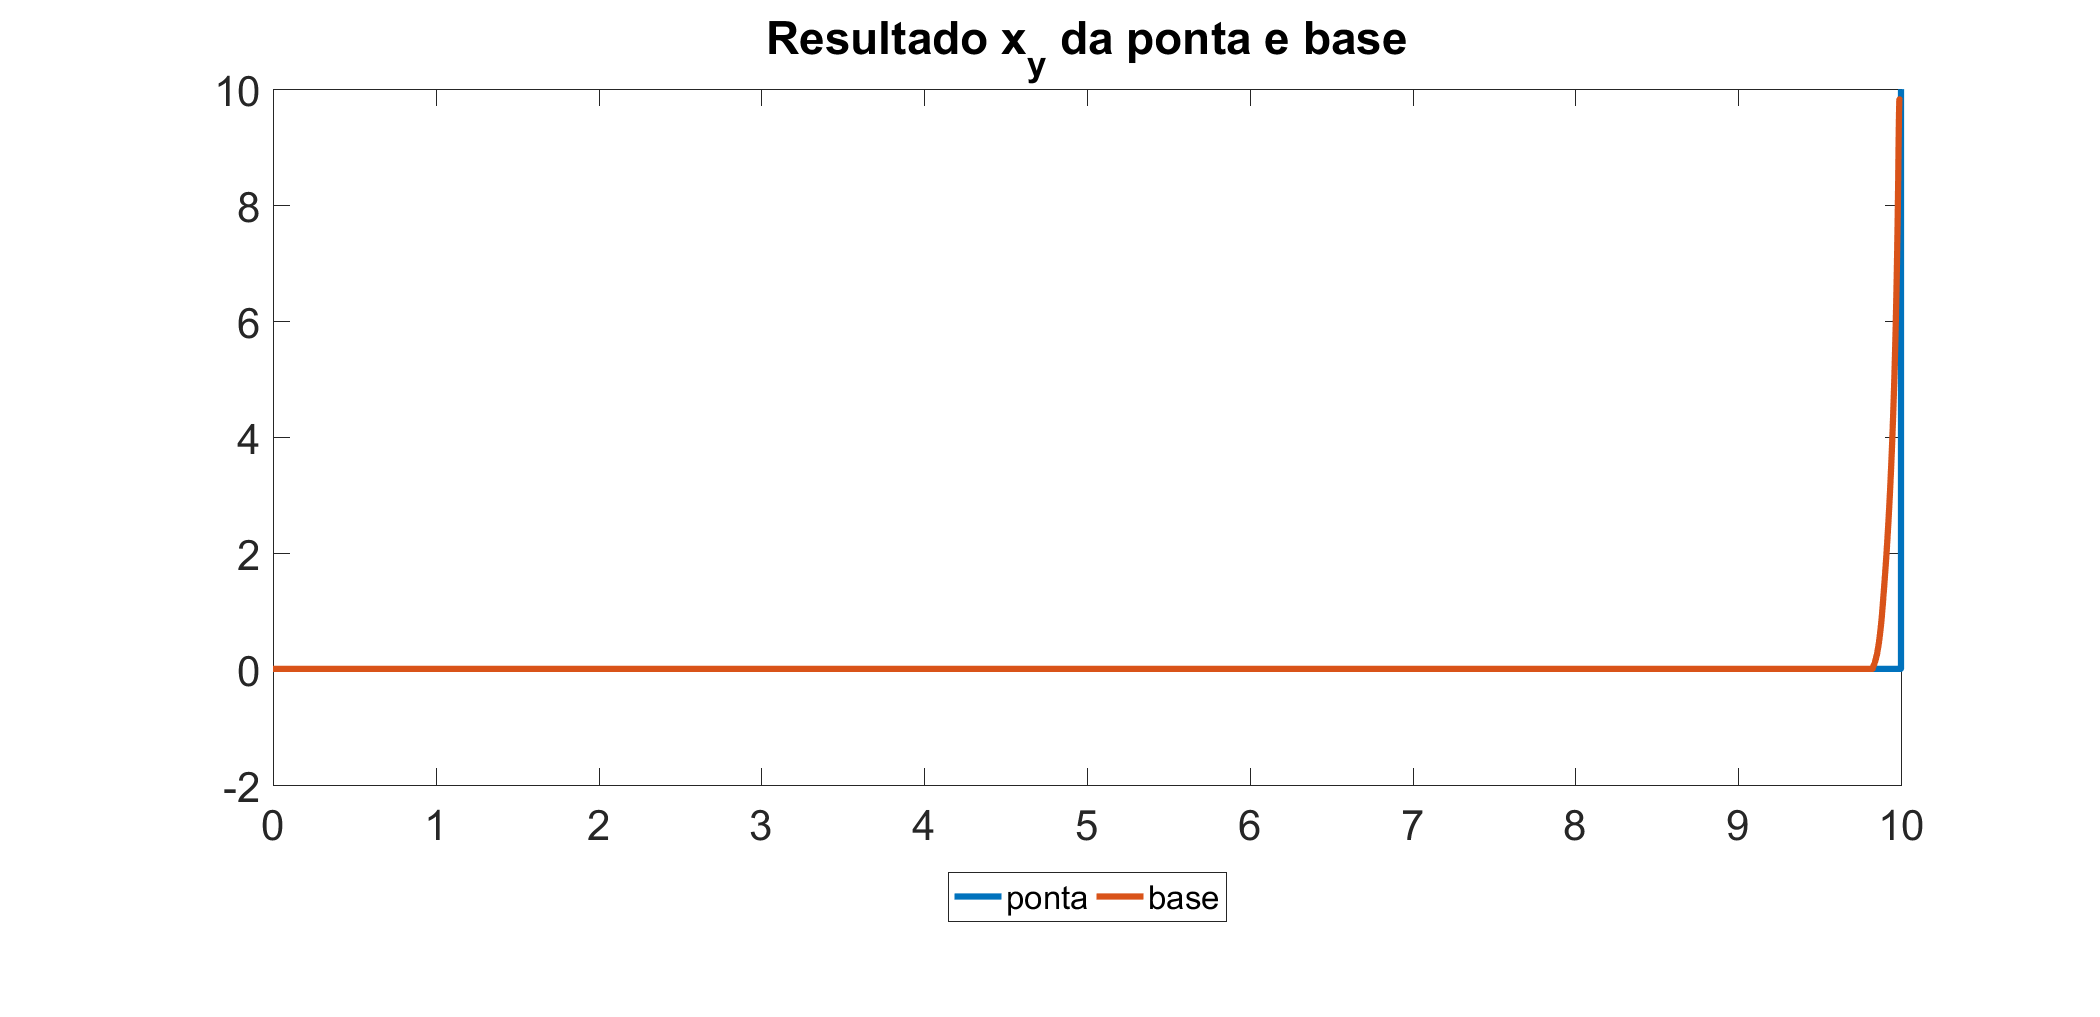
\includegraphics[scale=0.44]{Teste 2 C pos}
    \label{fig:t_2c_pos}
    \end{center}
\end{figure}

Curiosamente, o Caso A, que não conseguiu convergir e apresentou valores de entrada similares aos outros casos, serve como um exemplo notável de como variações no coeficiente de amortecimento podem levar a comportamentos divergentes. Este fenômeno é evidenciado na figura \ref{fig:t_2_viab}, onde observamos uma tendência de convergência para valores de viabilidade menores à medida que o coeficiente de amortecimento aumenta. Isso sugere uma maior facilidade em compensar desvios quando o coeficiente é elevado.

\begin{figure}[H]
    \begin{center}
    \caption{Caso 2 - Num de fun x Viabilidade}
    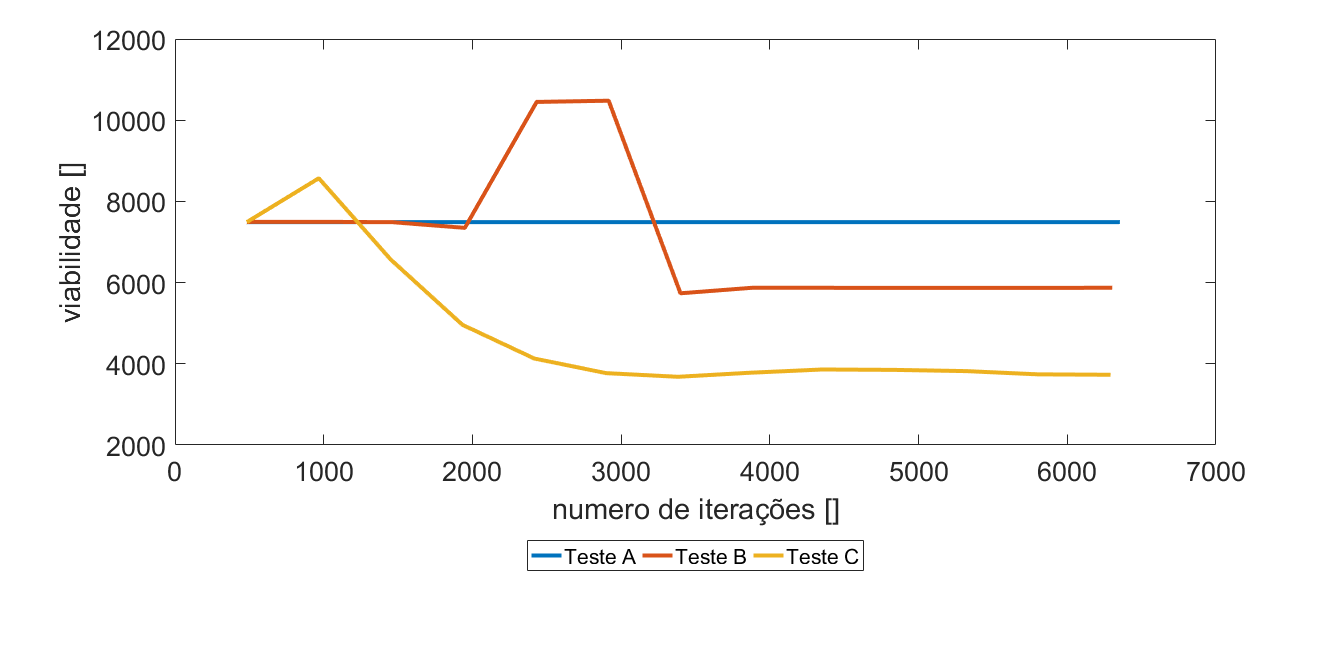
\includegraphics[scale=0.44]{Teste 2 Viabilidade}
    \label{fig:t_2_viab}
    \end{center}
\end{figure}

Em termos de desempenho computacional, todos os casos mantiveram uma consistência, com 241 elementos nos vetores de posição. Os tempos de simulação foram de 69, 89 e 52 segundos para os Casos 2A, 2B e 2C, respectivamente. Estes resultados indicam que, apesar das variações no coeficiente de amortecimento, a simulação manteve uma eficiência computacional comparável entre os diferentes casos.

\subsection{Caso 3 - Variação na aceleração}
Neste caso, focamos na influência da variação da aceleração na geração de comandos do sistema. A figura \ref{fig:t_3a_vels} é central nesta análise, pois ela revela uma forma distinta na curva de velocidade. Com a redução da aceleração, a velocidade não atingiu o patamar desejado, resultando em uma curva com formato triangular. Este comportamento destaca a sensibilidade do sistema às mudanças na aceleração e como isso afeta a capacidade de atingir velocidades alvo.

\begin{figure}[H]
    \begin{center}
    \caption{Caso 3A - Comportamento no tempo das velocidades em x e y da ponta e da referência}
    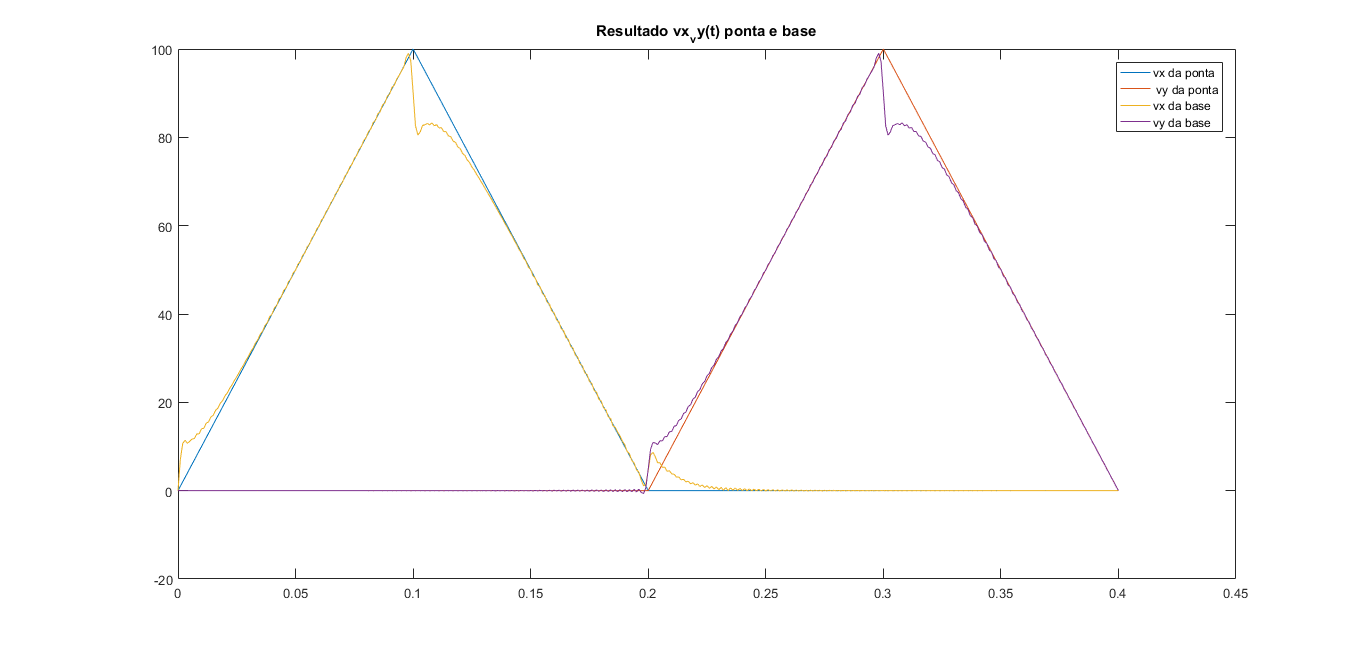
\includegraphics[scale=0.44]{Teste 3 A vels}
    \label{fig:t_3a_vels}
    \end{center}
\end{figure}

A figura \ref{fig:t_3_viab} fornece uma visão adicional sobre as dificuldades encontradas no Caso A. Ao contrário do Caso B, que mostrou um padrão de resposta semelhante aos casos anteriores, o Caso A enfrentou desafios significativos, como evidenciado por um aumento nos valores de viabilidade. Esta discrepância sugere que as variações na aceleração têm um impacto considerável na capacidade do sistema de satisfazer as restrições impostas.

\begin{figure}[H]
    \begin{center}
    \caption{Caso 3 - Num de fun x Viabilidade}
    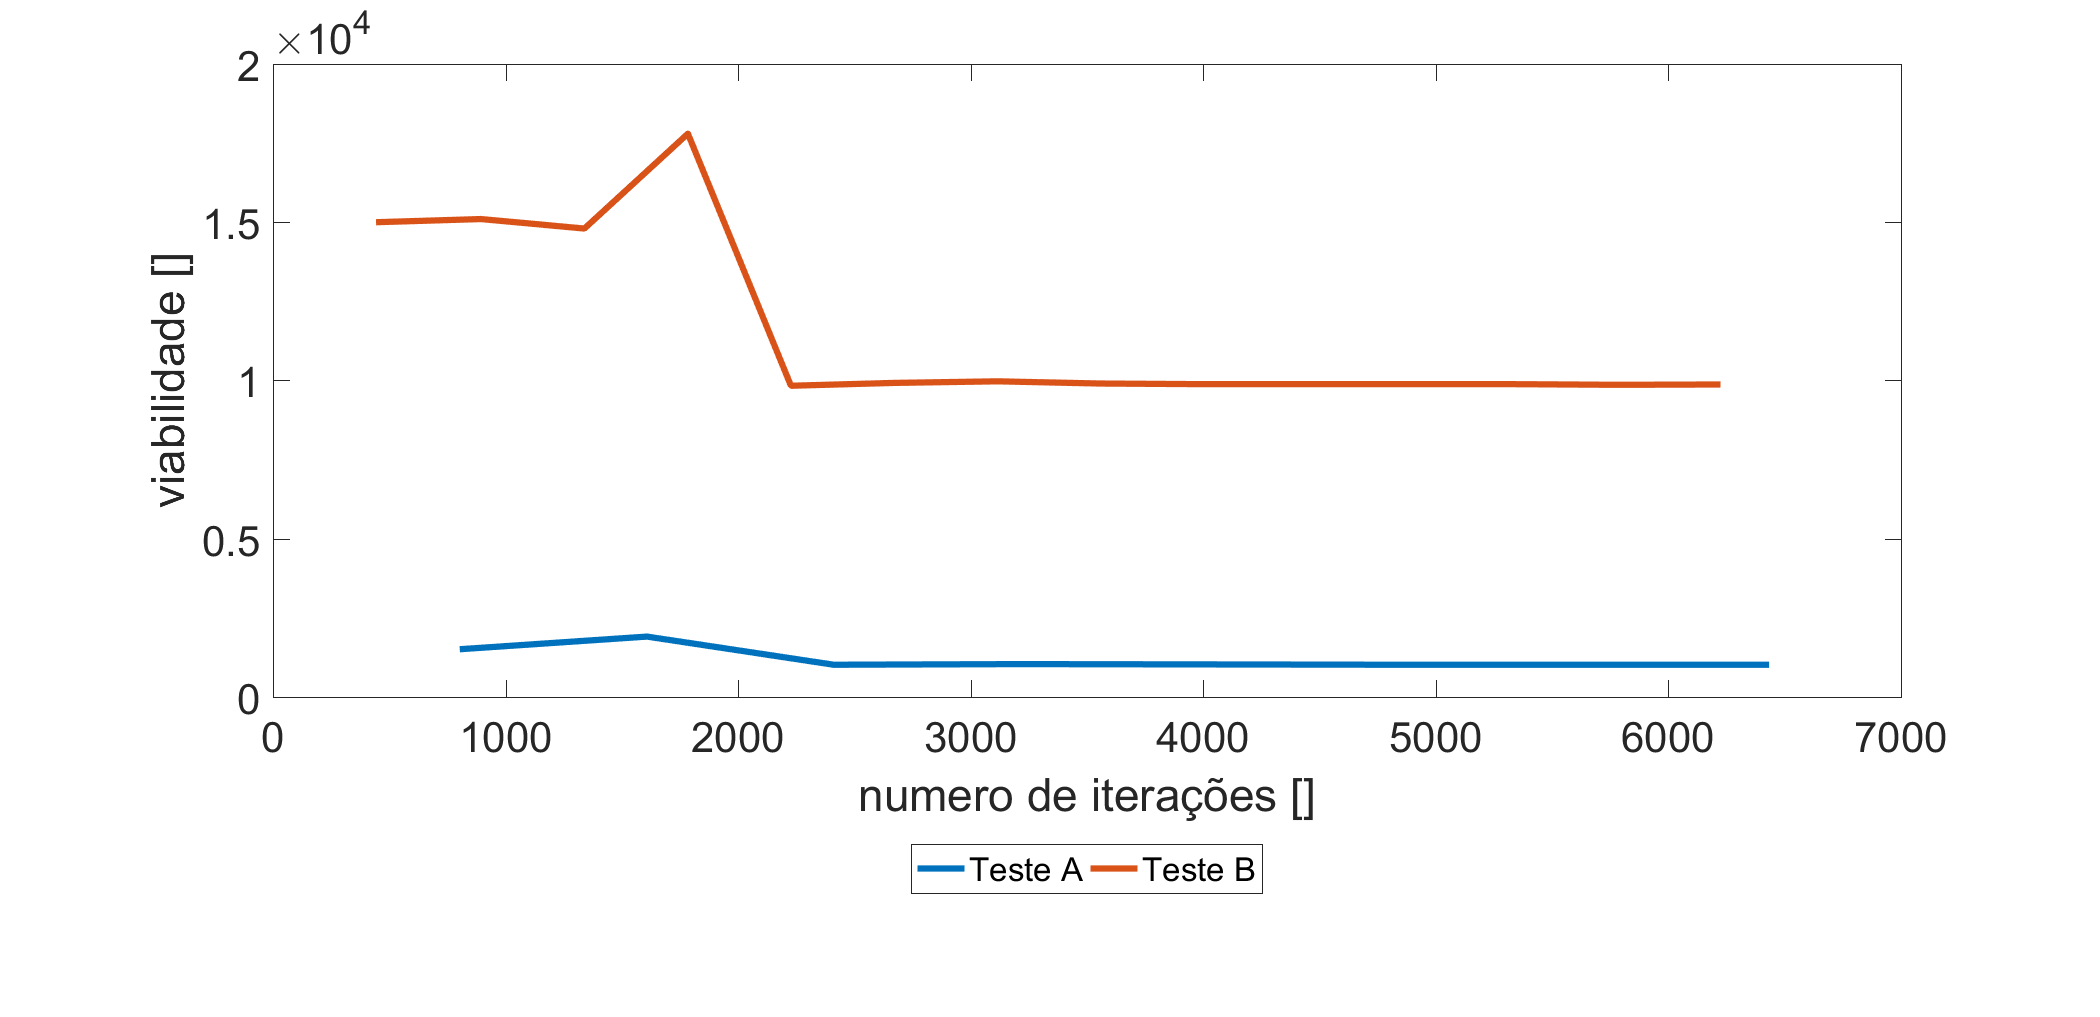
\includegraphics[scale=0.44]{Teste 3 Viabilidade}
    \label{fig:t_3_viab}
    \end{center}
\end{figure}

Uma possível explicação para as dificuldades observadas no Caso A pode ser encontrada no tamanho dos vetores de posição utilizados. No Caso A, o vetor de posições tinha 401 elementos e a simulação levou 195 segundos para ser concluída. Em contraste, o Caso B utilizou um vetor de 221 elementos e completou a simulação em 78 segundos. Estes resultados indicam que ajustes na aceleração podem ter implicações significativas não apenas no desempenho do sistema, mas também na eficiência computacional da simulação.

\subsection{Caso 4 - Variação dos passos de tempo}
Este caso destaca como diferentes resoluções na malha de tempo afetam o comportamento do sistema. As figuras \ref{fig:t_5a_vels}, \ref{fig:t_5b_vels} e \ref{fig:t_5c_vels} são fundamentais para entender a influência deste parâmetro nas oscilações observadas nos gráficos de velocidade. Cada uma destas figuras representa um cenário distinto, evidenciando como a resolução da malha de tempo pode alterar as dinâmicas de velocidade do sistema.

\begin{figure}[H]
    \begin{center}
    \caption{Caso 4A - Comportamento no tempo das velocidades em x e y da ponta e da referência}
    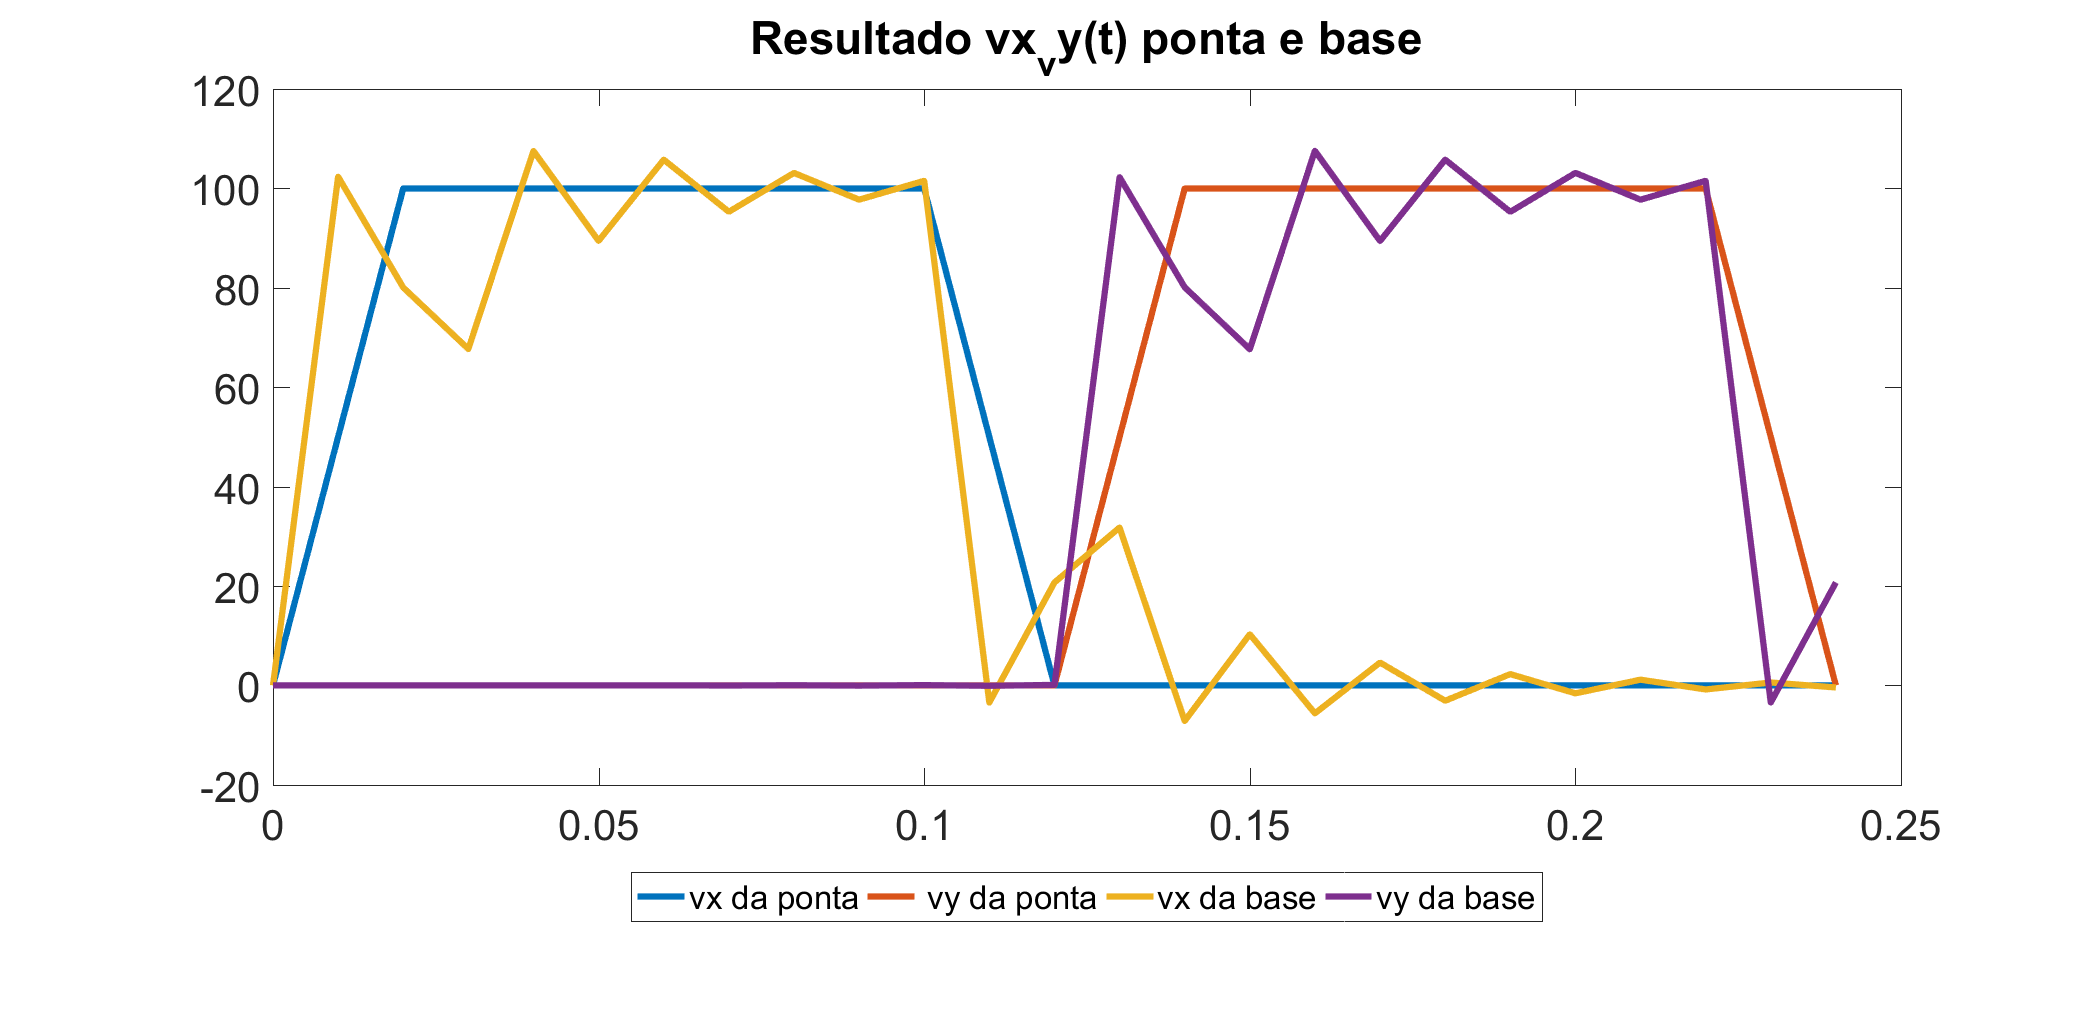
\includegraphics[scale=0.44]{Teste 5 A vels}
    \label{fig:t_5a_vels}
    \end{center}
\end{figure}

\begin{figure}[H]
    \begin{center}
    \caption{Caso 4B - Comportamento no tempo das velocidades em x e y da ponta e da referência}
    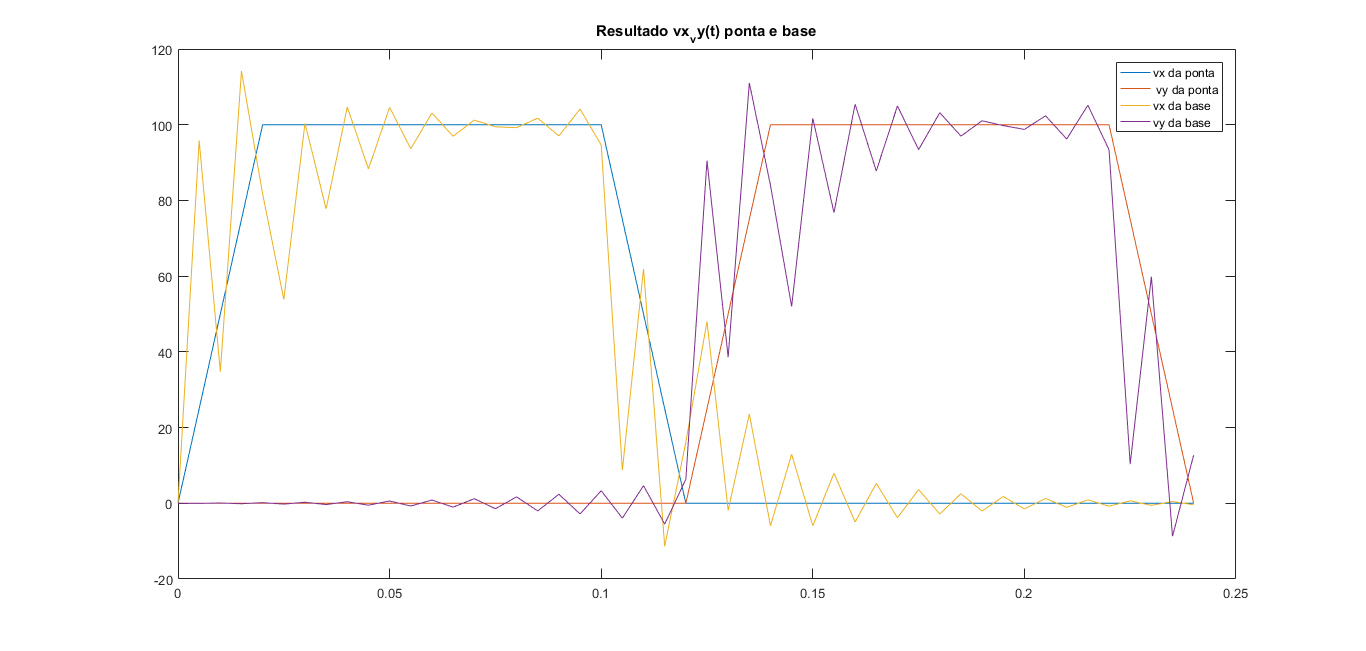
\includegraphics[scale=0.44]{Teste 5 B vels}
    \label{fig:t_5b_vels}
    \end{center}
\end{figure}

\begin{figure}[H]
    \begin{center}
    \caption{Caso 4C - Comportamento no tempo das velocidades em x e y da ponta e da referência}
    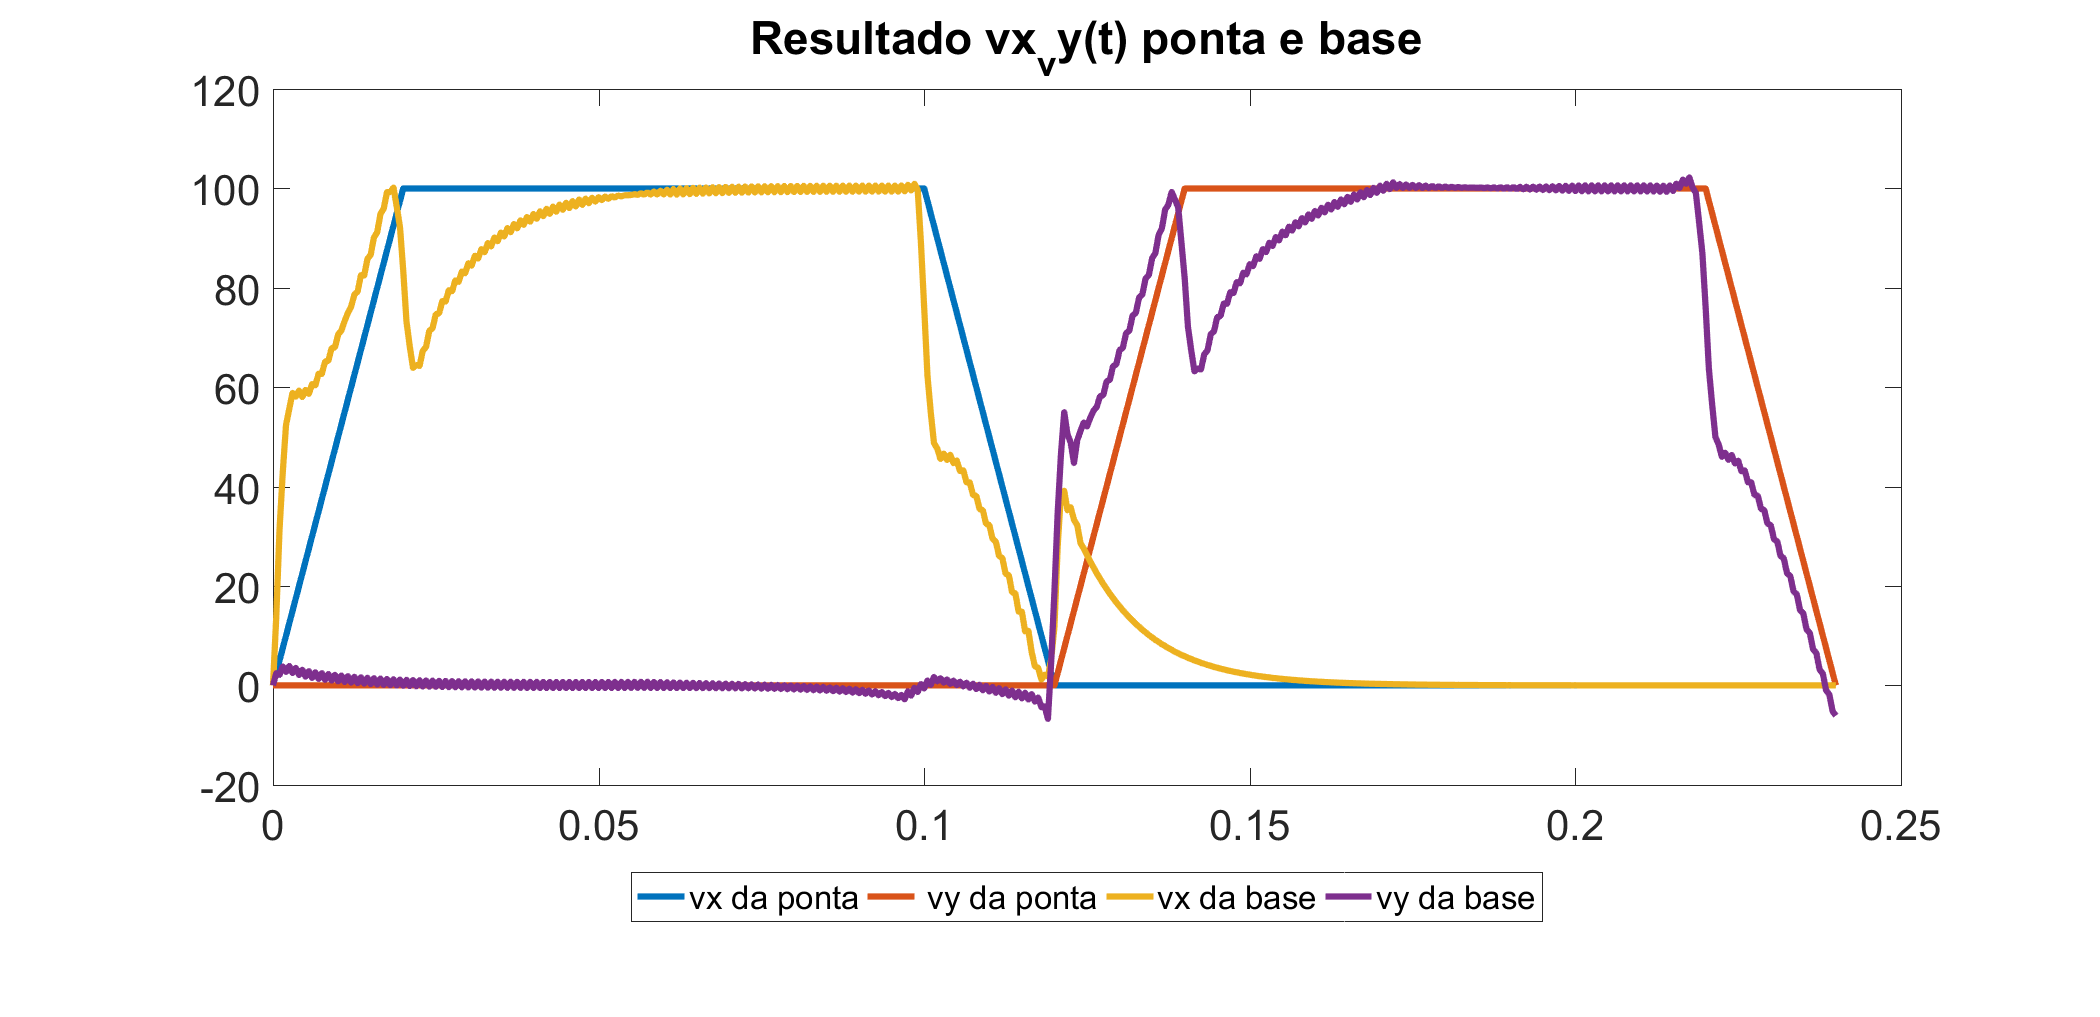
\includegraphics[scale=0.44]{Teste 5 C vels}
    \label{fig:t_5c_vels}
    \end{center}
\end{figure}

Por outro lado, ao examinar os gráficos de deslocamento nas figuras \ref{fig:t_5a_des}, \ref{fig:t_5b_des} e \ref{fig:t_5c_des}, notamos que as diferenças são menos pronunciadas. Isso sugere que, embora a resolução da malha de tempo tenha um impacto significativo na velocidade, seu efeito nos deslocamentos é mais sutil.

\begin{figure}[H]
    \begin{center}
    \caption{Caso 4A - Comportamento no tempo dos deslocamentos em x e y da ponta e da referência}
    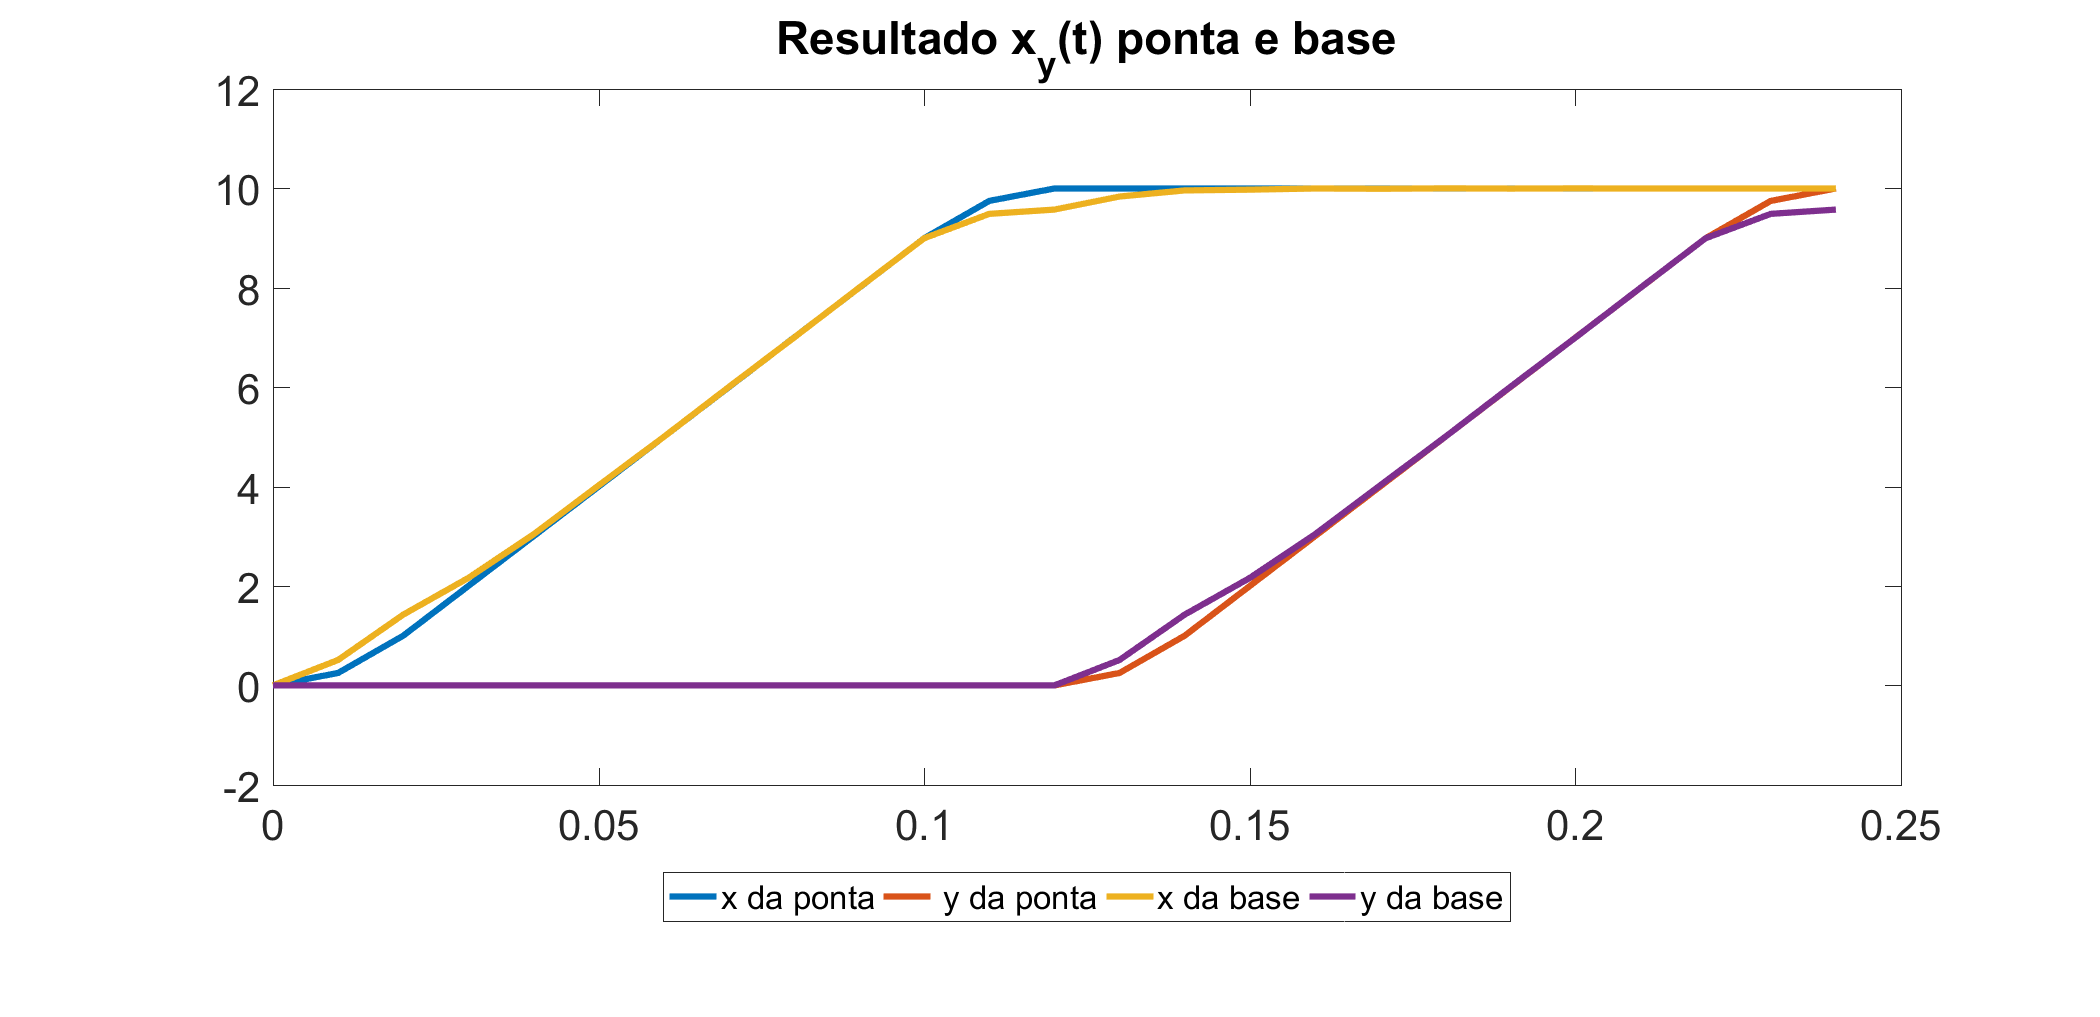
\includegraphics[scale=0.44]{Teste 5 A des}
    \label{fig:t_5a_des}
    \end{center}
\end{figure}

\begin{figure}[H]
    \begin{center}
    \caption{Caso 4B - Comportamento no tempo dos deslocamentos em x e y da ponta e da referência}
    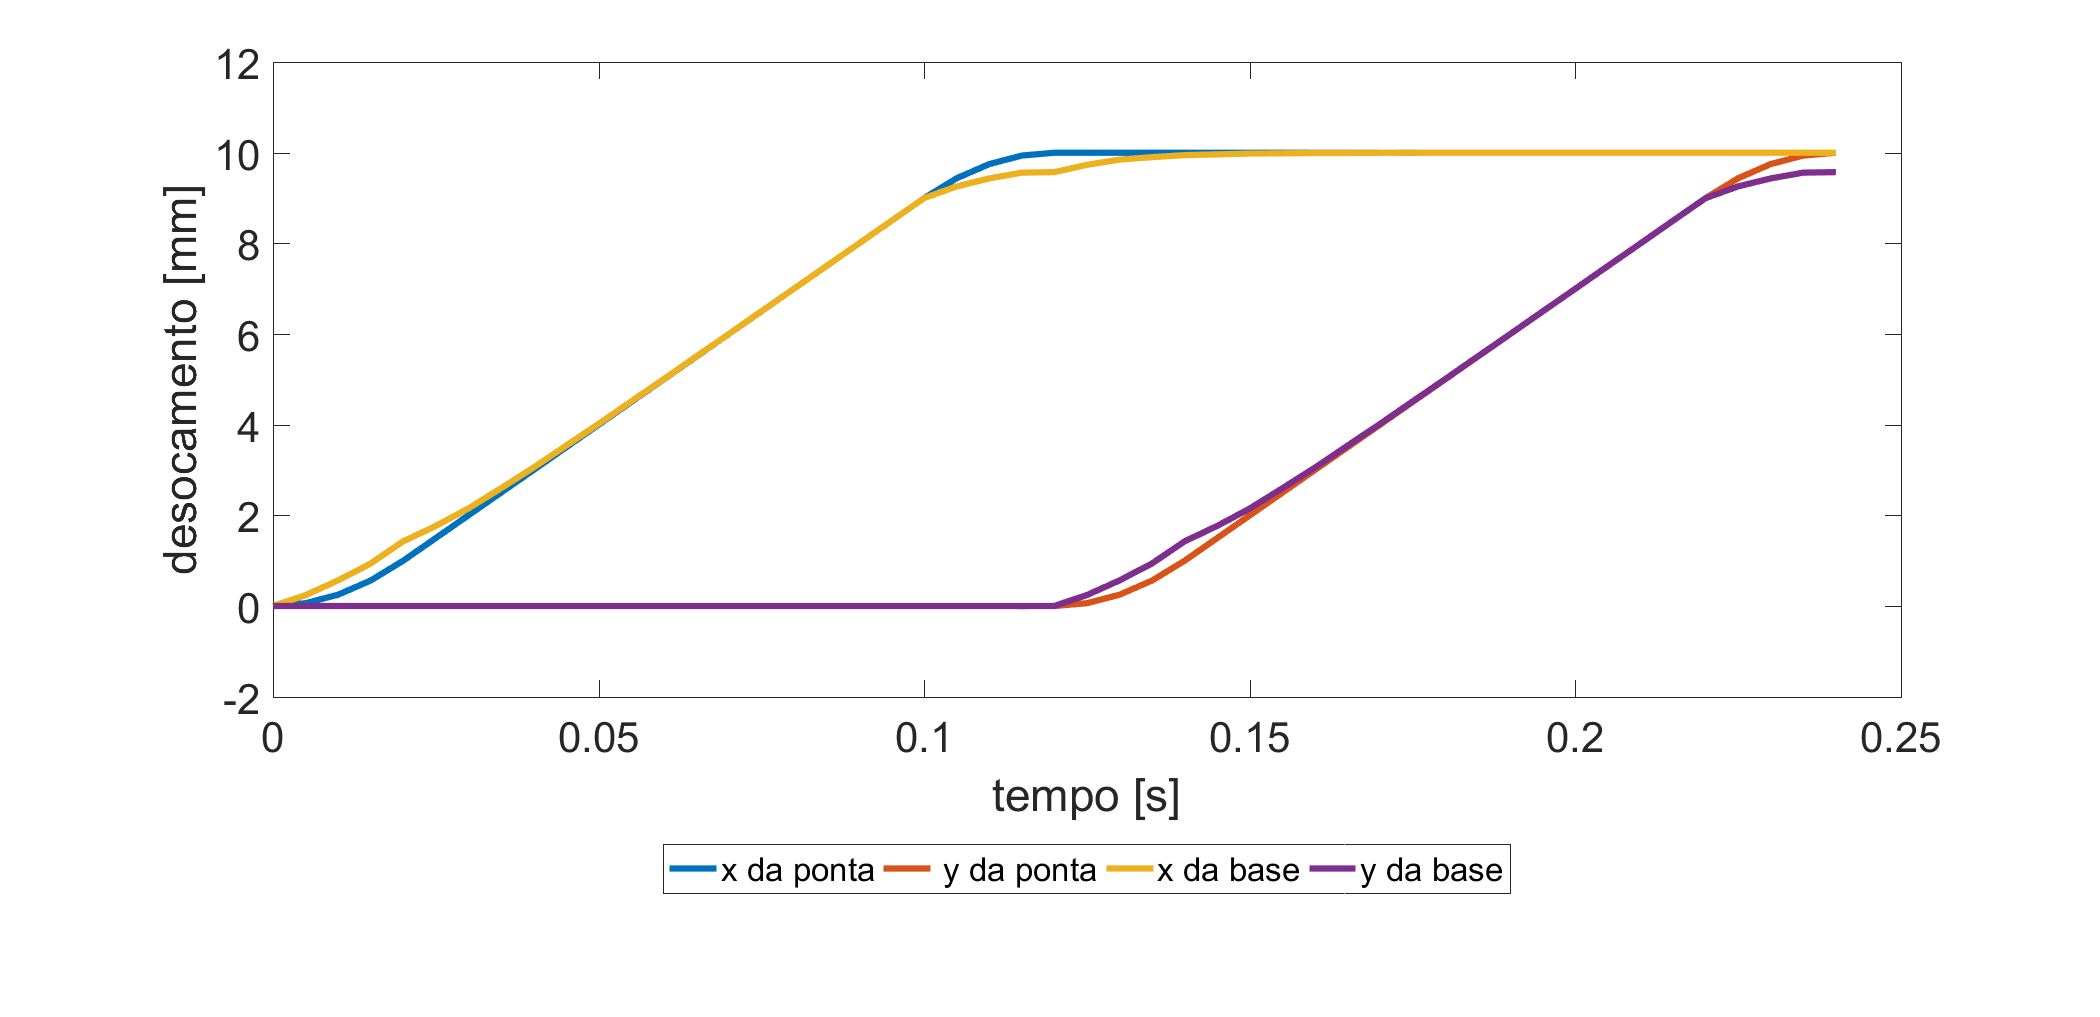
\includegraphics[scale=0.44]{Teste 5 B des}
    \label{fig:t_5b_des}
    \end{center}
\end{figure}

\begin{figure}[H]
    \begin{center}
    \caption{Caso 4C - Comportamento no tempo dos deslocamentos em x e y da ponta e da referência}
    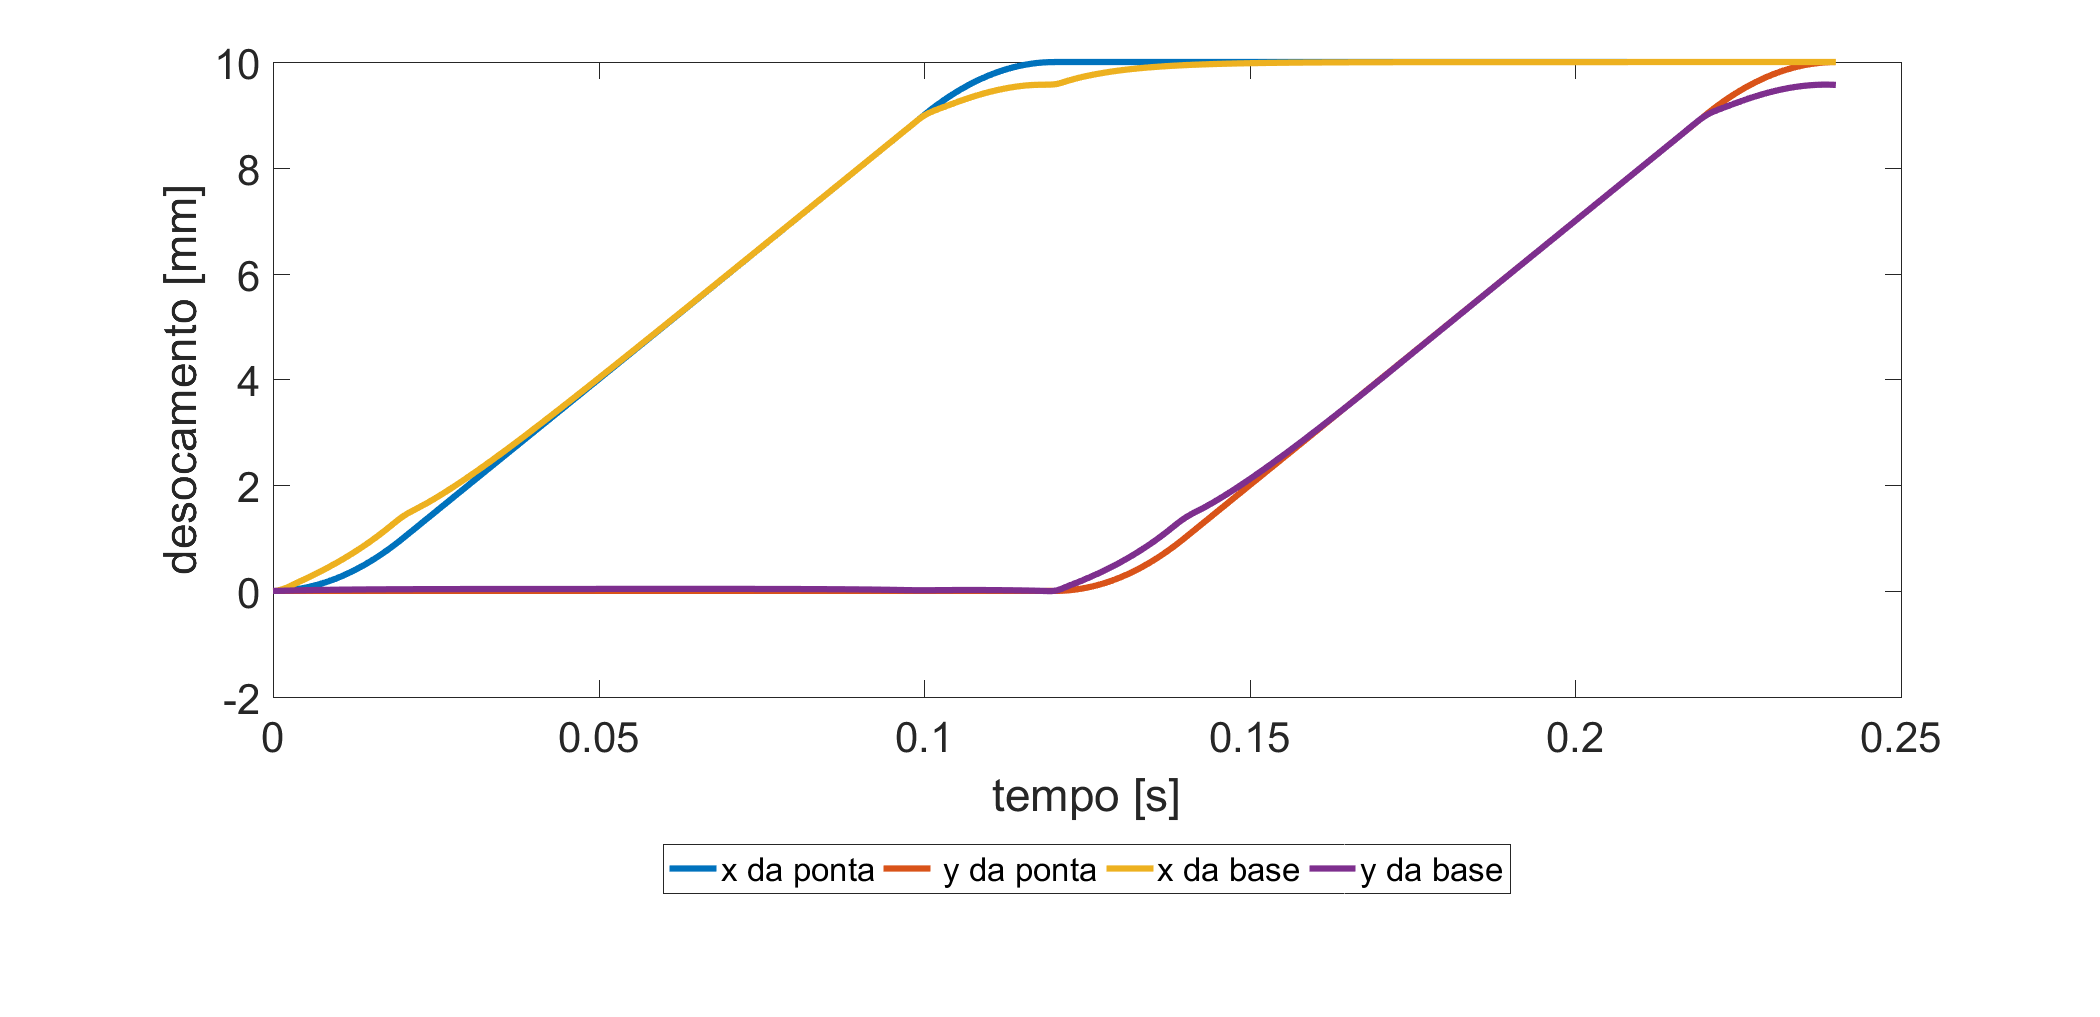
\includegraphics[scale=0.44]{Teste 5 C des}
    \label{fig:t_5c_des}
    \end{center}
\end{figure}

Além disso, a figura \ref{fig:t_5_viab} revela o impacto dessas variações na viabilidade da simulação, sugerindo uma relação entre a resolução da malha de tempo e a eficácia do sistema em alcançar a convergência. Os tempos de simulação variaram consideravelmente entre os casos, sendo 0,7 segundos para o Caso A, 3 segundos para o Caso B e 279 segundos para o Caso C. Este padrão de tempo está diretamente relacionado ao tamanho dos vetores de posição, que foram de 25, 49 e 481 elementos, respectivamente, para os Casos A, B e C.

\begin{figure}[H]
    \begin{center}
    \caption{Caso 4 - Num de fun x Viabilidade}
    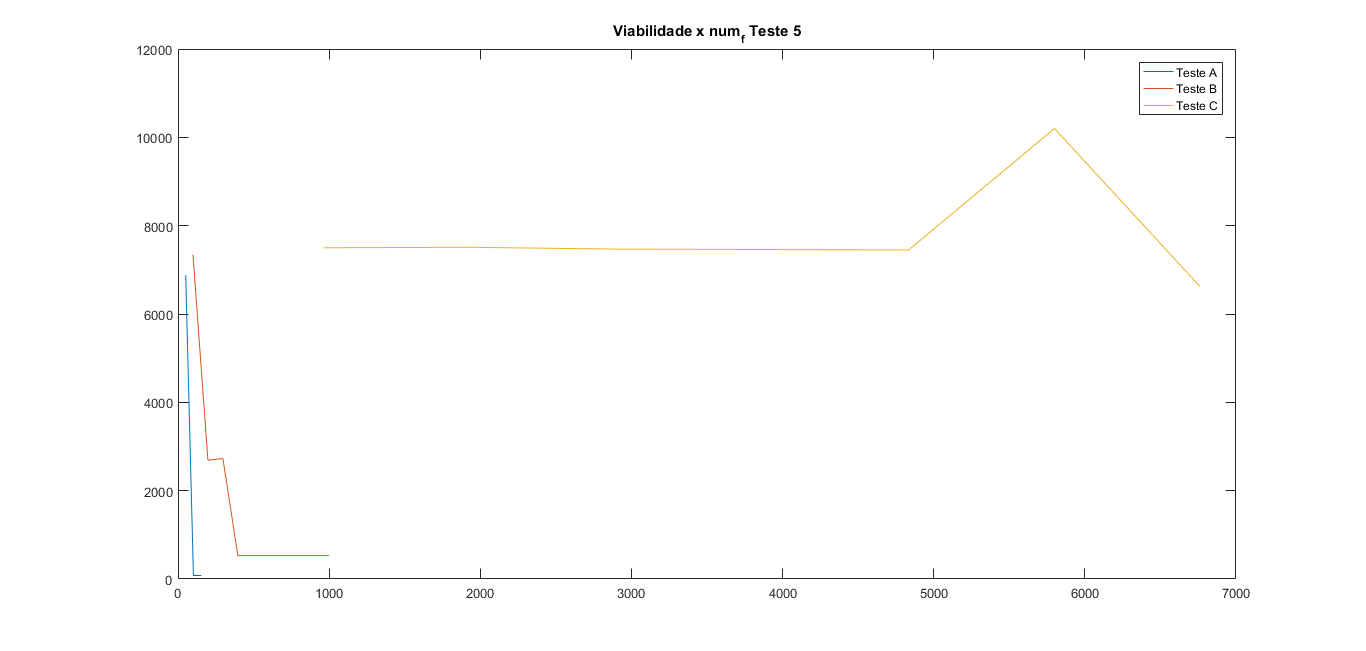
\includegraphics[scale=0.44]{Teste 5 Viabilidade}
    \label{fig:t_5_viab}
    \end{center}
\end{figure}

Podemos notar também o impacto na velocidade e facilidade de se convergir, podendo ser observado na figura \ref{fig:t_5_viab}, assim
como os tempos de simulação $0,7 s$, $3 s$ e $279 s$ para os Casos A, B e C respectivamente. Além do tamanho dos vetores que está diretamente relacionado,
respectivamente em 25, 49 e 481 para os Casos A, B e C.
\subsection{Caso 5 - Variação da velocidade}
Este caso foca na análise dos impactos causados por diferentes velocidades desejadas, ajustadas através do Gcode de entrada. Investigamos como as velocidades mais baixas e mais altas influenciam a dinâmica do sistema, tanto em termos de desempenho quanto de eficiência computacional.

No Caso A, onde a velocidade desejada é mais baixa, notamos um impacto significativo no tamanho dos vetores e no tempo de simulação. Devido à menor velocidade, o sistema leva mais tempo para completar o percurso, resultando em uma malha mais densa de pontos, dada a resolução de \(dt\) constante. Isso se traduz em um tempo de simulação mais longo de 219 segundos e 421 elementos nos vetores de posição.

Em contraste, o Caso B, com uma velocidade desejada mais alta, apresentou um tempo de simulação substancialmente menor de 60 segundos e 181 elementos nos vetores de posição. Interessante notar que, apesar da maior velocidade desejada e da manutenção da mesma aceleração máxima na geração de comando, a curva de velocidade neste caso assemelha-se à observada no Caso 3A, como mostrado na Figura \ref{fig:t_4b_vels}. A correspondente curva de deslocamento é ilustrada na Figura \ref{fig:t_4b_des}, destacando as diferenças no comportamento do sistema sob essas condições.

\begin{figure}[H]
    \begin{center}
    \caption{Caso 5B - Comportamento no tempo das velocidades em x e y da ponta e da referência}
    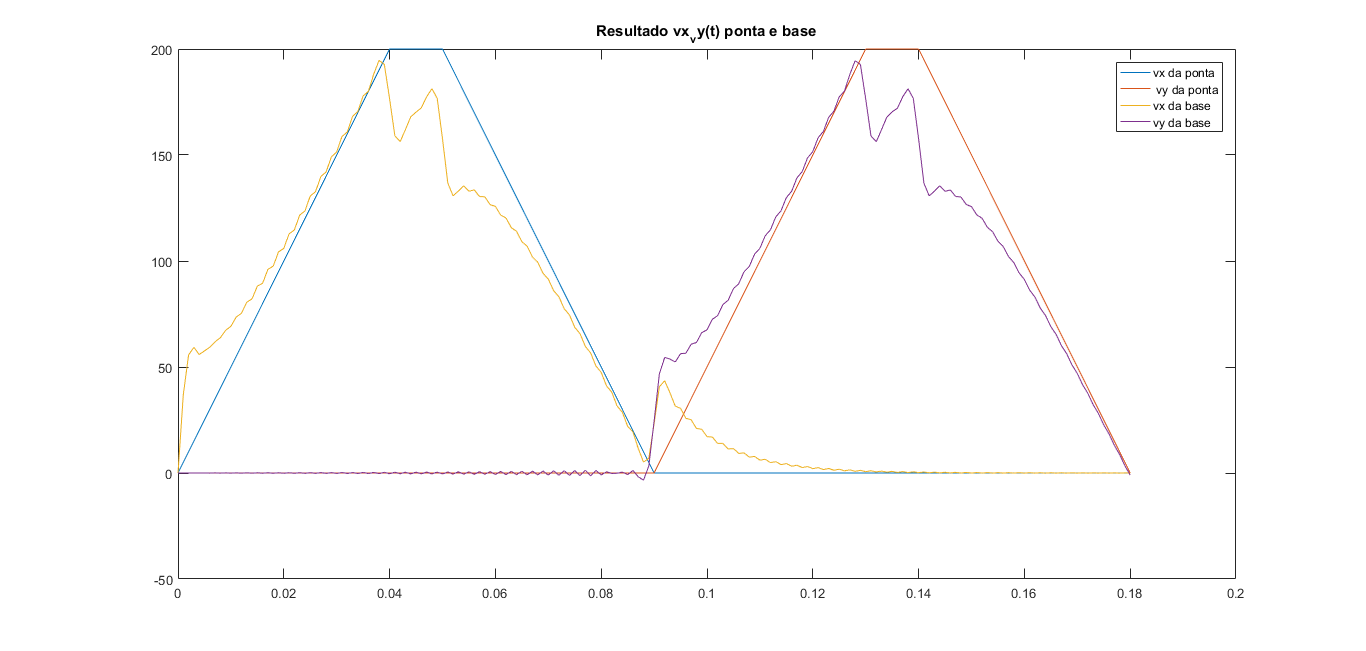
\includegraphics[scale=0.44]{Teste 4 B vels}
    \label{fig:t_4b_vels}
    \end{center}
\end{figure}

\begin{figure}[H]
    \begin{center}
    \caption{Caso 5B - Comportamento no tempo dos deslocamentos em x e y da ponta e da referência}
    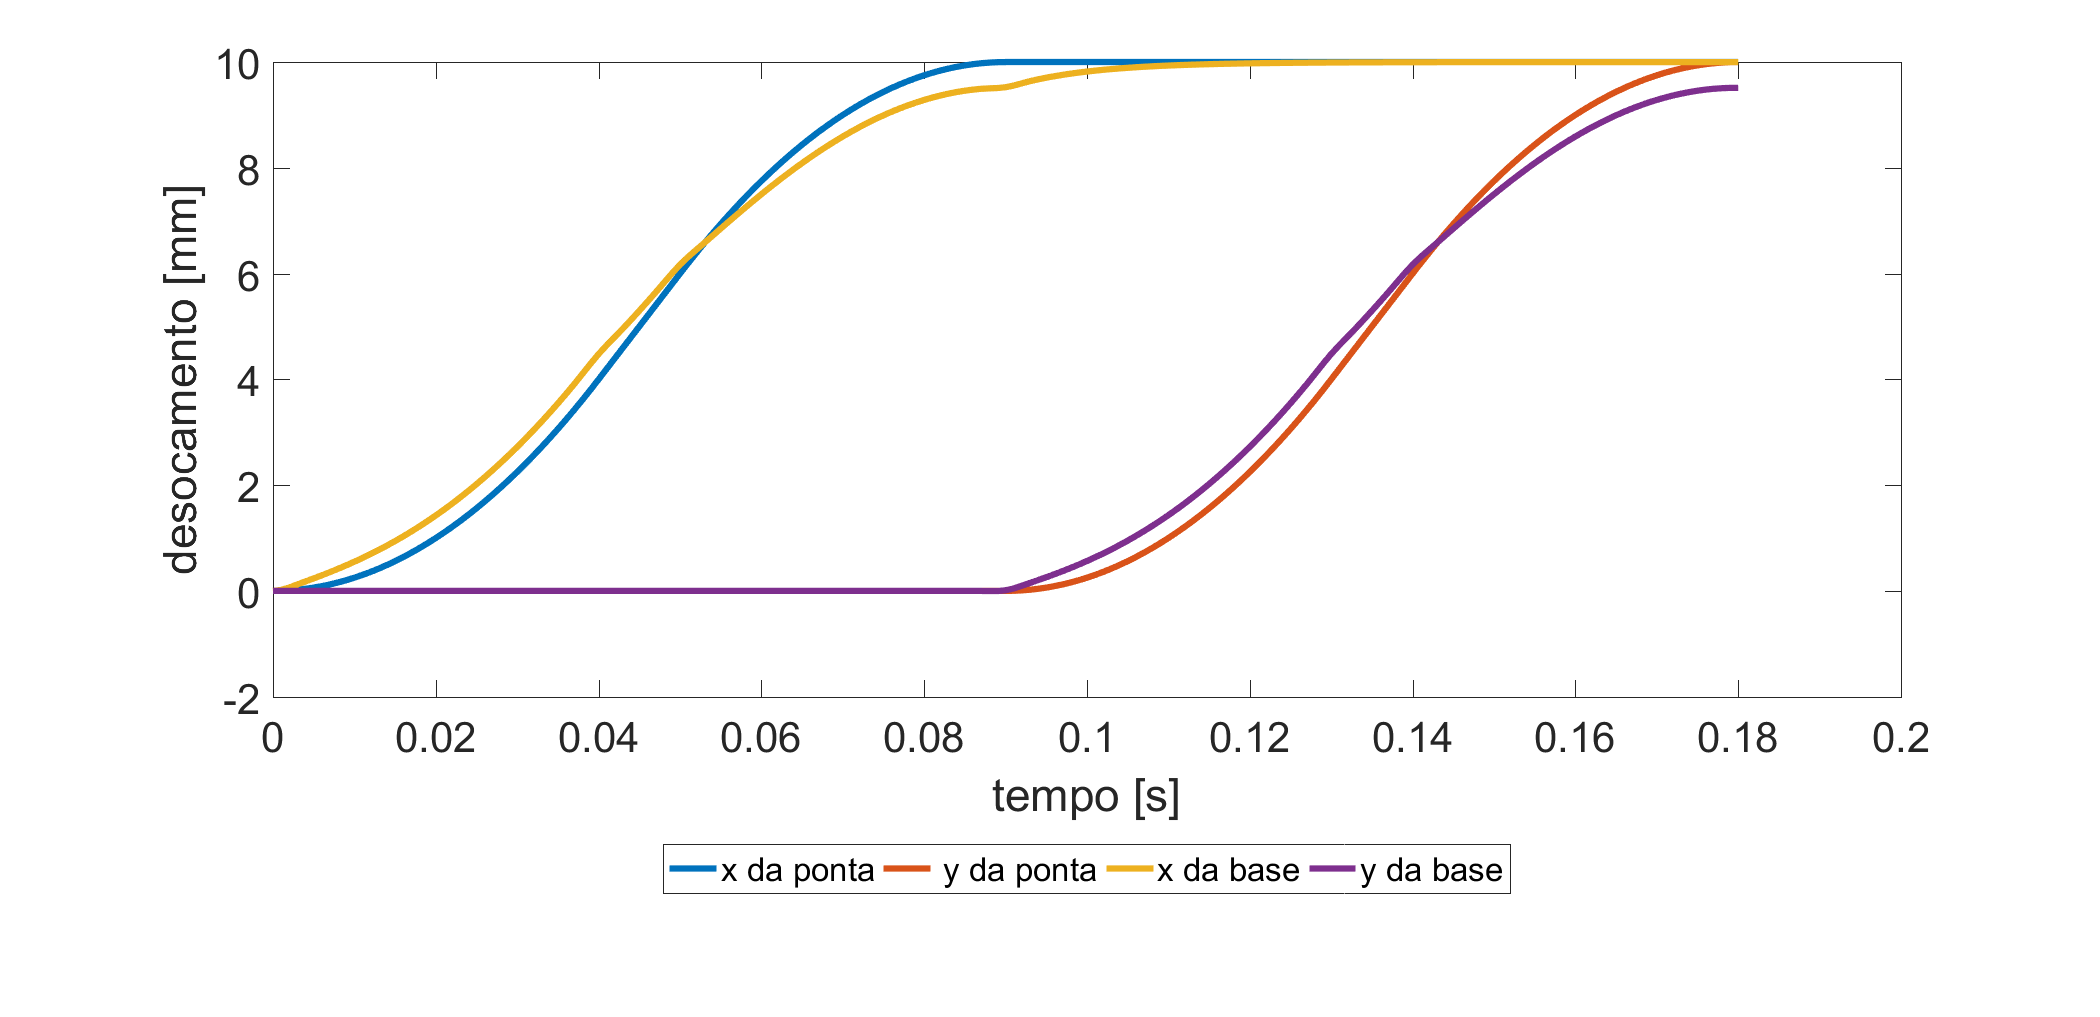
\includegraphics[scale=0.44]{Teste 4 B des}
    \label{fig:t_4b_des}
    \end{center}
\end{figure}

Além disso, a figura \ref{fig:t_4_viab} permite uma comparação do padrão de convergência em diferentes velocidades. Observa-se uma variação na viabilidade e na capacidade de o sistema atender às restrições impostas, variando de acordo com a velocidade configurada.

\begin{figure}[H]
    \begin{center}
    \caption{Caso 5 - Num de fun x Viabilidade}
    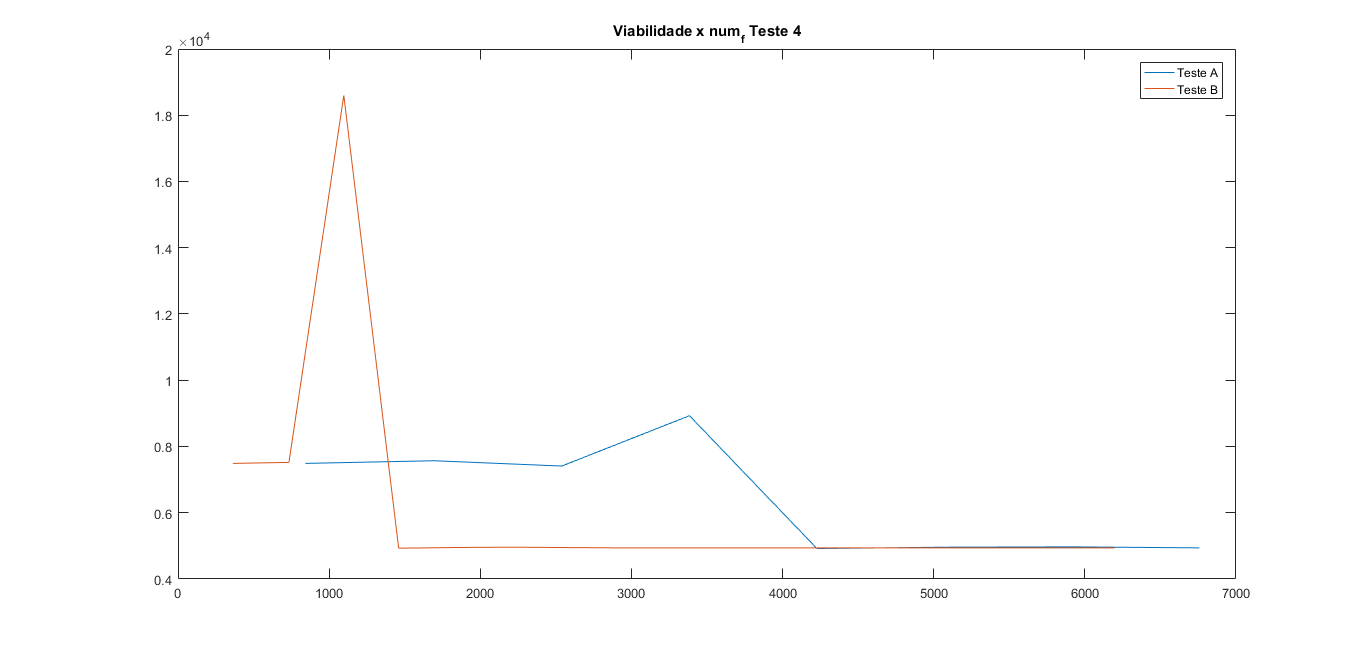
\includegraphics[scale=0.44]{Teste 4 Viabilidade}
    \label{fig:t_4_viab}
    \end{center}
\end{figure}

\section{Discussão Integrada dos Resultados}
Esta seção oferece uma análise integrada dos resultados obtidos nos diferentes casos de estudo, considerando as variáveis-chave e suas influências no comportamento do sistema simulado. A discussão foca em identificar padrões comuns, divergências e as implicações práticas dos resultados obtidos.

\subsection{Influência dos Parâmetros Variáveis}
A análise de sensibilidade realizada nos Casos 1 a 5 revelou que variações em parâmetros específicos, como frequência natural, coeficiente de amortecimento, aceleração, resolução de malha de tempo e velocidade desejada, têm impactos significativos e distintos no comportamento do sistema. 

No Caso 1, observou-se que a variação da frequência natural afeta diretamente a amplitude dos desvios e a necessidade de compensação. O Caso 2 mostrou que diferentes coeficientes de amortecimento podem levar a variações notáveis na trajetória e na viabilidade do sistema. No Caso 3, a alteração da aceleração demonstrou como esse parâmetro pode influenciar a forma da curva de velocidade e a eficiência da simulação. O Caso 4 destacou a importância da resolução da malha de tempo, especialmente em relação às oscilações de velocidade. Por fim, o Caso 5 ilustrou como a velocidade desejada afeta tanto o tempo de simulação quanto o tamanho dos vetores de posição.

\subsection{Comportamento e Convergência do Sistema}
Em todos os casos, observou-se uma tendência de convergência para soluções viáveis, embora com variações na velocidade e facilidade desta convergência. Notavelmente, os casos com maiores desafios em termos de convergência e viabilidade foram aqueles com maiores variações nos parâmetros estudados. Isso sugere que, enquanto o sistema é robusto e adaptável a uma ampla gama de condições, existem limites críticos além dos quais a eficácia do sistema começa a diminuir.

\subsection{Considerações futuras}
Uma possível abordagem a ser explorada utilizando a ideia do método deste trabalho é a sobreposição de algoritmos, onde
um método referenciado em uma planta do sistema poderia buscar remover uma parcela das vibrações, atuando de forma estagiada,
com a participação de um método como \textit{InputShaping} para atacar as vibrações remanescentes.

Uma possibilidade que o tipo de método abordado neste trabalho oferece é a capacidade de otimizar os parâmetros da planta para uma determinada posição.
Assim, oferecendo a capacidade de se ajustar em grande nível de detalhe as peculiaridades do sistema, podendo até
construir a malha utilizando sensores, semelhantemente a rotinas de configuração de \textit{InputShaping} que amostram
o comportamento em frequência no ponto central da impressora. Considerando também que a utilização desse tipo de malha,
teria pouco impacto computacional.



\chapter{CONCLUSÃO}
Esta monografia apresentou um método de controle de trajetória para sistemas de impressão 3D, focado em aprimorar a precisão do posicionamento da ferramenta. A implementação do método demonstrou uma diminuição notável no desvio do caminho da ponta quando comparado ao caminho simulado sem controle de trajetória.

Os resultados obtidos por meio de simulações confirmaram a capacidade do controle em atenuar as complexidades dinâmicas do sistema. A simulação de referência, juntamente com as simulações de parâmetros variados, validou a eficácia do algoritmo de controle sob diferentes condições operacionais.

A análise dos parâmetros do sistema, incluindo frequência natural, coeficiente de amortecimento, aceleração de entrada, passo de tempo e velocidade desejada, permitiu quantificar sua influência na resposta do controle e teve resultados esperados indicando uma concordância verossímil com os modelos estabelecidos.

A pesquisa identificou a importância de ajustar o passo de tempo de acordo com a frequência natural para uma representação mais fiel da resposta do sistema e indicou a execução do controle de trajetória em etapas de diferentes passos de tempo como uma abordagem efetiva para aprimorar o processo de controle.

Em síntese, as contribuições deste trabalho para o campo do controle de trajetória são evidenciadas pela melhoria na precisão da impressão 3D dada pelas simulações e contribui para a exploração de métodos iterativos e de programação linear, estabelecendo um ponto de partida para futuros avanços na otimização de sistemas de controle no contexto de impressoras 3D.

%==============================================================================
% Incluindo bibliografia
%\bibliographystyle{plain}             % estilo para labels em numeros
%\bibliographystyle{alpha}             % estilo para labels em iniciais
\bibliographystyle{abntex2-alf}           % estilo para referências usando ABNT, 
                                       % precisa instalar o abntex para usar!!!

%inclui Referências Bibliográficas
%inclui Referências Bibliográficas
\referencias
%\bibliography{refbib}			% arquivo exemplo refbib.bib
%==============================================================================
% Incluindo anexos num1erados com letras maiusculas.
%\apendices


%==============================================================================
% Fim do texto
\end{document}
